%% ========================
%  Kurzanleitung:
%  Diese Datei ist die Hauptdatei, die mit dem TeX-Programm geöffnet wird. 
%  Wird empfehlen dazu TeXStudio.
%  
%  Außer in dem mit Pfeilen markierten Bereich etwas weiter unten
%  sollte in dieser Datei nicht geändert werden.
%  
%  Die Grundeinstellungen (Titel der Arbeit, Name, Formatiertungsdetails)
%  können in der Datei "einstellungen.tex" vorgenommen werden.
% 
%  Die ursprüngliche Version dieser Vorlage wurde erstellt durch 
%  die Fakultät Informatik der TU Dortmund. Die vorliegende Version wurde 
%  modifiziert durch den Lehrstuhl 13. 
%% ========================

%% ========================
%  Zwei Konfigurationsdateien, die selbst keinen Text-Inhalt enthalten.
%  "header.tex" sollte unverändert bleiben.
%  "einstellungen.tex" muss editiert werden.
%% ========================
% header.tex
\documentclass[a4paper,12pt,ngerman]{article}
% Dimensionen des Dokuments. Nicht ändern!
%\usepackage[a4paper,left=3.5cm,right=2.5cm,bottom=2.5cm,top=3.5cm,headheight=20pt]{geometry}

\usepackage[pdftex]{graphicx}

% Einige wichtige Standard-Pakete
\usepackage{amsmath,amssymb,subfigure}

% Theorem-Umgebungen
\usepackage[amsmath,thmmarks]{ntheorem}

% Korrekte Darstellung der Umlaute
\usepackage[utf8x]{inputenc}
\usepackage[ngerman]{babel}
\usepackage[T1]{fontenc}

% Minimale Verbesserung von Zeilenumbrüchen und Wortabständen
\usepackage{microtype}

% Formatierung von floats
\usepackage{floatrow}

% Algorithmen
\usepackage[plain,chapter]{algorithm}
\usepackage{algorithmic}

\usepackage{enumerate}
% Eine verbesserte Version der Schriftart computer modern; für Vektorschrift überall.
\usepackage{lmodern}

% Bibtex deutsch
\usepackage{bibgerm}

% Für Testzwecke
\usepackage{blindtext}

% urls
\usepackage[hidelinks, colorlinks=true, urlcolor=blue]{hyperref}

% Umfließender Text neben Bild
\usepackage{wrapfig}

% Multirow für Tabellen
\usepackage{multirow}

% Eurosymbol
\usepackage{eurosym}

% Zeilenabstand
\usepackage{setspace}

% Caption Packet
\usepackage[margin=0pt,font=small,labelfont=bf]{caption}

\usepackage[explicit]{titlesec}

%Für das Einbinden der Eidestattlichen Erklärung
\usepackage{pdfpages}

% Das fancy header paket für schönere Kopf- und Fußzeilen
\usepackage{fancyhdr}
\usepackage{helvet}
\usepackage{xcolor}
\usepackage{calc}

\usepackage{svg}

% ==============
% Es folgt die Konfiguration der Kopf- und Fußzeilen
% ==============
\definecolor{TUGreen}{rgb}{0.517,0.721,0.094}
\definecolor{bgpagenum}{gray}{.75}
\definecolor{fgheader}{gray}{.6}
\newboolean{TuFarben}
\setboolean{TuFarben}{false}


\def\mystrut(#1){\vrule height #1pt width 0pt}    
\newlength{\headerspace}
\setlength{\headerspace}{1mm}

\newboolean{KopfInnen}
\setboolean{KopfInnen}{false}

\newcommand{\textmarkleft}{\fontfamily{phv}\selectfont\fontsize{12}{5}\bfseries
	\colorbox{bgpagenum}{
		\begin{minipage}[t][8pt]{4cm}
		\raggedleft\textcolor{white}{\thepage}
		\end{minipage}
	}
	\hspace{\headerspace}
	\textcolor{fgheader}{
		\nouppercase\rightmark
	}
}
	
\newcommand{\textmarkright}{
	\fontfamily{phv}\selectfont\fontsize{12}{5}\bfseries
	\textcolor{fgheader}{
		\nouppercase\leftmark
	}
	\hspace{\headerspace}
	\colorbox{bgpagenum}{
		\begin{minipage}[t][8pt]{4cm}
			\raggedright\textcolor{white}{\thepage}	
		\end{minipage}
	}
}

\newcommand{\numbermarkright}{
	\fontfamily{phv}\selectfont\fontsize{12}{5}\bfseries
	\colorbox{bgpagenum}{
		\begin{minipage}[t][8pt]{4cm}
			\raggedright\textcolor{white}{\thepage}
		\end{minipage}
	}
}

\newcommand{\numbermarkleft}{
	\fontfamily{phv}\selectfont\fontsize{12}{5}\bfseries
	\colorbox{bgpagenum}{
		\begin{minipage}[t][8pt]{4cm}
			\raggedleft\textcolor{white}{\thepage}	
		\end{minipage}
	}
}

\newcommand{\fancypages}{
	\pagestyle{fancy}
	\ifthenelse{\boolean{KopfInnen}}{
		\fancyheadoffset[loh]{4.5cm}
		\fancyheadoffset[reh]{4.5cm}
	}{
		\fancyheadoffset[leh]{4.5cm}
		\fancyheadoffset[roh]{4.5cm}
	}
	\renewcommand{\headrulewidth}{0pt}
	\renewcommand{\footrulewidth}{0pt}
	\fancyhead[LO]{\ifthenelse{\boolean{KopfInnen}}{\textmarkleft}{}}
	\fancyhead[RO]{\ifthenelse{\boolean{KopfInnen}}{}{\textmarkright}}
	\fancyhead[RE]{\ifthenelse{\boolean{KopfInnen}}{\textmarkright}{}}
	\fancyhead[LE]{\ifthenelse{\boolean{KopfInnen}}{}{\textmarkleft}}
	\fancyfoot[C]{}
}

\newcommand{\configurefancypages}{
	\fancypagestyle{plain}{%
		\fancyhf{} 
		\ifthenelse{\boolean{KopfInnen}}{
			\fancyheadoffset[loh]{4.5cm}
			\fancyheadoffset[reh]{4.5cm}
		}{
			\fancyheadoffset[leh]{4.5cm}
			\fancyheadoffset[roh]{4.5cm}
		}
		\renewcommand{\headrulewidth}{0pt}
		\renewcommand{\footrulewidth}{0pt}
		
		\fancyhead[LO]{\ifthenelse{\boolean{KopfInnen}}{\numbermarkleft}{}}
		\fancyhead[RO]{\ifthenelse{\boolean{KopfInnen}}{}{\numbermarkright}}
		\fancyhead[RE]{\ifthenelse{\boolean{KopfInnen}}{\numbermarkright}{}}
		\fancyhead[LE]{\ifthenelse{\boolean{KopfInnen}}{}{\numbermarkleft} }
		\fancyfoot[C]{}
	}
	\ifthenelse{\boolean{TuFarben}}{
		\colorlet{bgpagenum}{TUGreen!70!white}
		\colorlet{fgheader}{TUGreen!80!white}
	}{}
}
% ==============
% Konfiguration der Kopf- und Fußzeilen abgeschlossen.
% ==============


% Konfiguration der Chapter-Überschriften 
% für den Fall, dass ausgefallene Überschriften gewünscht sind
\newboolean{UnterlegteKapitel}
\setboolean{UnterlegteKapitel}{false}
\newlength{\almosttextwidth}
\setlength{\almosttextwidth}{\textwidth-6pt}
\newcommand{\configurechapterheadings}{
\ifthenelse{\boolean{UnterlegteKapitel}}{
	
	\titleformat{\chapter}
	{\vspace{-0.75cm}\normalfont\Huge\bfseries}{}{0em}{\colorbox{bgpagenum}{\begin{minipage}[b][60pt]{\almosttextwidth}\strut\textcolor{white}{\thechapter\quad##1}\end{minipage}}}
	\titleformat{name=\chapter,numberless}
	{\vspace{-0.75cm}\normalfont\Huge\bfseries}{}{0em}{\colorbox{bgpagenum}{\begin{minipage}[b][60pt]{\almosttextwidth}\strut\textcolor{white}{##1}\end{minipage}}}
}{}
}

% Einige Einstellungen für Floats. Bitte nicht ändern!
\floatsetup[table]{capposition=top}
\floatsetup[algorithm]{capposition=top}

% Theorem-Optionen %
\theoremseparator{.}
\theoremstyle{change}
\newtheorem{theorem}{Theorem}[section]
\newtheorem{satz}[theorem]{Satz}
\newtheorem{lemma}[theorem]{Lemma}
\newtheorem{korollar}[theorem]{Korollar}
\newtheorem{proposition}[theorem]{Proposition}
% Ohne Numerierung
\theoremstyle{nonumberplain}
\renewtheorem{theorem*}{Theorem}
\renewtheorem{satz*}{Satz}
\renewtheorem{lemma*}{Lemma}
\renewtheorem{korollar*}{Korollar}
\renewtheorem{proposition*}{Proposition}
% Definitionen mit \upshape
\theorembodyfont{\upshape}
\theoremstyle{change}
\newtheorem{definition}[theorem]{Definition}
\theoremstyle{nonumberplain}
\renewtheorem{definition*}{Definition}
% Kursive Schrift
\theoremheaderfont{\itshape}
\newtheorem{notation}{Notation}
\newtheorem{konvention}{Konvention}
\newtheorem{bezeichnung}{Bezeichnung}
\theoremsymbol{\ensuremath{\Box}}
\newtheorem{beweis}{Beweis}
\theoremsymbol{}
\theoremstyle{change}
\theoremheaderfont{\bfseries}
\newtheorem{bemerkung}[theorem]{Bemerkung}
\newtheorem{beobachtung}[theorem]{Beobachtung}
\newtheorem{beispiel}[theorem]{Beispiel}
\newtheorem{problem}{Problem}
\theoremstyle{nonumberplain}
\renewtheorem{bemerkung*}{Bemerkung}
\renewtheorem{beispiel*}{Beispiel}
\renewtheorem{problem*}{Problem}

\newcommand{\kooperation}{}

% Algorithmen anpassen %
\renewcommand{\algorithmicrequire}{\textit{Eingabe:}}
\renewcommand{\algorithmicensure}{\textit{Ausgabe:}}
\floatname{algorithm}{Algorithmus}
\renewcommand{\listalgorithmname}{Algorithmenverzeichnis}
\renewcommand{\algorithmiccomment}[1]{\color{grau}{// #1}}

% Zeilenabstand einstellen %
\renewcommand{\baselinestretch}{1.25}
% Floating-Umgebungen anpassen %
\renewcommand{\topfraction}{0.9}
\renewcommand{\bottomfraction}{0.8}
% Abkuerzungen richtig formatieren %
\usepackage{xspace}
\newcommand{\vgl}{vgl.\@\xspace} 
\newcommand{\zB}{z.\nolinebreak[4]\hspace{0.125em}\nolinebreak[4]B.\@\xspace}
\newcommand{\bzw}{bzw.\@\xspace}
\newcommand{\dahe}{d.\nolinebreak[4]\hspace{0.125em}h.\nolinebreak[4]\@\xspace}
\newcommand{\etc}{etc.\@\xspace}
\newcommand{\evtl}{evtl.\@\xspace}
\newcommand{\ggf}{ggf.\@\xspace}
\newcommand{\bzgl}{bzgl.\@\xspace}
\newcommand{\so}{s.\nolinebreak[4]\hspace{0.125em}\nolinebreak[4]o.\@\xspace}
\newcommand{\iA}{i.\nolinebreak[4]\hspace{0.125em}\nolinebreak[4]A.\@\xspace}
\newcommand{\sa}{s.\nolinebreak[4]\hspace{0.125em}\nolinebreak[4]a.\@\xspace}
\newcommand{\su}{s.\nolinebreak[4]\hspace{0.125em}\nolinebreak[4]u.\@\xspace}
\newcommand{\ua}{u.\nolinebreak[4]\hspace{0.125em}\nolinebreak[4]a.\@\xspace}
\newcommand{\og}{o.\nolinebreak[4]\hspace{0.125em}\nolinebreak[4]g.\@\xspace}
\newcommand{\oBdA}{o.\nolinebreak[4]\hspace{0.125em}\nolinebreak[4]B.\nolinebreak[4]\hspace{0.125em}d.\nolinebreak[4]\hspace{0.125em}A.\@\xspace}
\newcommand{\OBdA}{O.\nolinebreak[4]\hspace{0.125em}\nolinebreak[4]B.\nolinebreak[4]\hspace{0.125em}d.\nolinebreak[4]\hspace{0.125em}A.\@\xspace}

% Leere Seite ohne Seitennummer, naechste Seite rechts
% Für Titelseite nötig, sonst nicht.
\newcommand{\blankpage}{
 \clearpage{\pagestyle{empty}\cleardoublepage}
}

%Booleans, die die Formatierung der Verzeichnisse im Anhang bestimmen
\newboolean{AbbildungsverzeichnisEinfuegen}
\newboolean{AlgorithmenverzeichnisEinfuegen}
\newboolean{TabellenverzeichnisEinfuegen}
\newboolean{PlatzsparendeVerzeichnisse}

% Keine einzelnen Zeilen beim Anfang eines Abschnitts (Schusterjungen)
\clubpenalty = 10000
% Keine einzelnen Zeilen am Ende eines Abschnitts (Hurenkinder)
\widowpenalty = 10000 \displaywidowpenalty = 10000
% EOF

\usepackage{moresize}

\usepackage{pifont}% http://ctan.org/pkg/pifont

\usepackage{listings}
\definecolor{deepblue}{rgb}{0,0,0.5}
\definecolor{deepred}{rgb}{0.6,0,0}
\definecolor{deepgreen}{rgb}{0,0.5,0}

\lstset{
	basicstyle=\small\ttfamily,
	numbers=left,
	showstringspaces=false,
	commentstyle=\color{red},
	keywordstyle=\color{blue}
}

%\newcommand\pythonstyle{\lstset{
\lstdefinestyle{myPython}{
	language=Python,
	basicstyle=\small,
	numbers=left,
	breaklines=true,
	tabsize=2,
	frame=lines,
	otherkeywords={self},             
	keywordstyle=\ttfamily\color{blue!90!black},
	keywords=[2]{True,False},
	keywords=[3]{ttk, row, column, sticky, fg, bg, font, lat, lon},
	keywordstyle={[2]\ttfamily\color{yellow!80!orange}},
	keywordstyle={[3]\ttfamily\color{red!80!orange}},
	emph={MyClass,__init__},          
	emphstyle=\ttfamily\color{red!80!black}, 
	stringstyle=\ttfamily\color{deepgreen},                        % Any extra options here
	showstringspaces=false            % 
	%}}
}

\colorlet{punct}{red!60!black}
\definecolor{background}{HTML}{EEEEEE}
\definecolor{delim}{RGB}{20,105,176}
\colorlet{numb}{magenta!60!black}

\lstdefinelanguage{json}{
	basicstyle=\ssmall\ttfamily,
	numbers=left,
	numberstyle=\ssmall,
	stepnumber=1,
	numbersep=8pt,
	showstringspaces=false,
	breaklines=true,
	frame=lines,
	backgroundcolor=\color{background},
	literate=
	*{0}{{{\color{numb}0}}}{1}
	{1}{{{\color{numb}1}}}{1}
	{2}{{{\color{numb}2}}}{1}
	{3}{{{\color{numb}3}}}{1}
	{4}{{{\color{numb}4}}}{1}
	{5}{{{\color{numb}5}}}{1}
	{6}{{{\color{numb}6}}}{1}
	{7}{{{\color{numb}7}}}{1}
	{8}{{{\color{numb}8}}}{1}
	{9}{{{\color{numb}9}}}{1}
	{:}{{{\color{punct}{:}}}}{1}
	{,}{{{\color{punct}{,}}}}{1}
	{\{}{{{\color{delim}{\{}}}}{1}
	{\}}{{{\color{delim}{\}}}}}{1}
	{[}{{{\color{delim}{[}}}}{1}
	{]}{{{\color{delim}{]}}}}{1},
}


%% ========================
% Globale Einstellungen. Müssen angepasst werden!
%% ========================
\newcommand{\erstgutachter}{Arno Pasternak}
\newcommand{\zweitgutachter}{Johannes Fischer}
\newcommand{\drittgutachter}{Johannes Pieper}
\newcommand{\autorname}{Timon Sachweh und Michael Ratke}
% Umbruch im Titel mit "\\"
\newcommand{\titel}{SmartMirror}
\newcommand{\arbeitstyp}{Ausarbeitung für das Proseminar: Raspberry Pi}
% Die nächste Zeile einkommentieren, falls die Nennung einer kooperierenden Entität gewünscht ist.
%\renewcommand{\kooperation}{In Kooperation mit:\\Firma/Fakultät/Lehrstuhl}

%% ========================
%  Einstellungen für Verzeichnisse.
%  Hier können die gewünschten Verzeichnisse im Anhang an- und abgestellt werden.
%% ========================
% Abbildungsverzeichnis einfügen?
\setboolean{AbbildungsverzeichnisEinfuegen}{true}
% Tabellenverzeichnis einfügen?
\setboolean{AlgorithmenverzeichnisEinfuegen}{false}
% Algorithmenverzeichnis einfügen?
\setboolean{TabellenverzeichnisEinfuegen}{false}
% Verzeichnisse im Anhang statt immer zweiseitig auch einseitig zulassen, um leere Seite zu vermeiden? Wenn die Verzeichnisse sehr wenig enthalten, sollte auf "true" geschaltet werden.
\setboolean{PlatzsparendeVerzeichnisse}{false}

%% ========================
%  Sollen Kopfzeilen innen oder außen dargestellt werden? 
%  Wenn der Drucker keinen Druck bis an den Seitenrand erlaubt 
%  (gilt für die meisten Heimanwender-Drucker), sollte "true" gewählt werden,
%  sonst (gilt i.d.R. für das Drucken im Copy-Shop) sollte "false" gewählt werden.
%% ========================
\setboolean{KopfInnen}{false}

%% ========================
%  Sollen aufwändige (farblich unterlegte) Kapitelüberschriften verwendet werden?
%% ========================
\setboolean{UnterlegteKapitel}{false}

%% ========================
%  Sollen für Kopfzeilen und Kapitelüberschriften TU-Farben verwendet werden?
%  (Gilt nur für aufwändige Kapitelüberschriften.)
%% ========================
\setboolean{TuFarben}{false}


%% ========================
%  Titelseite und Inhaltsverzeichnis
%  Hier nichts ändern!
%% ========================
\configurefancypages
\configurechapterheadings
\begin{document}
\pagenumbering{Alph}
\begin{titlepage}
\vspace*{-2cm}
\newlength{\links}
\setlength{\links}{-1.5cm}
\fontfamily{lmss}\selectfont
\LARGE

\hspace*{\links}
\begin{minipage}{12.5cm}

\includegraphics[width=8cm]{bilder/tud_logo_cmyk}
\end{minipage}

\vspace*{1.8cm}

\hspace*{-0.6cm}
\begin{minipage}[t][7.5cm][c]{7.5cm}
\large
\begin{center}

{\Large \arbeitstyp} \\
\vspace*{1cm}
\textbf{\titel } \\
\vspace*{1cm}
\autorname\\
\today
\end{center}
\end{minipage}


\vfill

\hspace*{\links}
\begin{minipage}[b]{8cm}
\normalsize
\raggedright
Gutachter: \\
\erstgutachter \\
\zweitgutachter \\
\vspace{1cm}
\normalsize
\raggedright
Fakultät für Informatik\\
Lehrstuhl für Dienstleistungsinformatik (LS13)\\
Technische Universität Dortmund \\
\url{http://ls13-www.cs.tu-dortmund.de}
\end{minipage}
\hspace{2cm}
\begin{minipage}[b]{5cm}
	\normalsize
	\raggedleft
	\kooperation
\end{minipage}

\end{titlepage}

%\blankpage
\pagenumbering{roman}
\microtypesetup{protrusion=false}
\pagestyle{plain}
\tableofcontents
\microtypesetup{protrusion=true}
%d\cleardoublepage
%\fancypages
\pagenumbering{arabic}

%% ========================
%  Ab hier folgt der eigentliche Inhalt der Arbeit.	
%  Hier können beliebige .tex-Dateien eingefügt werden.
%% ====================================================
%% ↓↓↓↓↓↓↓↓↓↓↓↓↓↓↓↓↓↓↓↓↓↓↓↓↓↓↓↓↓↓↓↓↓↓↓↓↓↓↓↓↓↓↓↓↓↓↓↓↓↓↓↓


% einleitung.tex
\chapter{Motivation und Einleitung}
Das aktuelle Trend der Digitalisierung zeichnet sich besonders dadurch aus, dass Alltagsgegenstände smart und miteinander vernetzt werden. Folglich entlasten diese den Menschen bei alltäglichen Aufgaben. Ein Beispiel dafür ist ein Saugroboter, der vollautomatisch eine gesamte Etage saugen kann.

Im Bezug auf die Menschen hat dieser Wandel in der globalisierten Welt die Auswirkung, dass leichtere Aufgaben von den elektrischen Geräten übernommen werden, sodass dem Menschen die Verpflichtung abgenommen wird. Im Umkehrschluss müssen Menschen zunehmend komplexere Entscheidungen treffen, die mit mehr Verantwortung einhergehen. 

Die zunehmende Globalisierung erhöht ebenfalls die Anforderungen an die zeitliche Verfügbarkeit der menschlichen Arbeitskraft bei steigender Entgrenzung von Lebens- und Arbeitswelt. Diese steigenden Anforderungen an die Menschen werden zunehmend durch technische Unterstützungssysteme kompensiert, da diese elektronische Geräte inzwischen kontextspezifische Informationen aufbereiten und übersichtlich visualisiert darstellen, sodass sie die Menschen bei ihren Aufgaben unterstützen und an Ereignisse erinnern können. Aus diesem Grund erfahren solche unterstützenden Systeme eine kontinuierlich wachsende Bedeutung.

In diesem Zusammenhang haben sich SmartMirrors als hilfreiche Geräte zur Datenvisualisierung und Unterstützung des Menschen herausgestellt. So liefern sie jederzeit die aktuellsten Nachrichten, damit der Besitzer immer auf dem aktuellen Stand des Weltgeschehens ist. Im besonderen können sie Demenz-kranken helfen, indem die wichtigsten Dinge, die ein Patient nicht vergessen darf, jederzeit über den SmartMirror abrufbar sind. Allerdings ist es wie häufig bei neuen oder medizinisch relevanten Produkten so, dass diese derzeit in einem hohen Preissegment liegen.

Aus diesem Grund ist es das Ziel dieser Ausarbeitung, zu zeigen, dass solch ein SmartMirror auch mit einem kleineren Budget und den Kenntnissen eines Informatikstudenten realisierbar ist.

Grundsätzlich ist die Ausarbeitung so aufgebaut, dass zunächst ein Überblick über die im Spiegel integrierten Hardwarekomponenten gegeben wird. Anschließend beschreibt die Ausarbeitung den Aufbau der Softwarekonstruktion und das Zusammenspiel zwischen Hardware und Software. Ein Resümee über den Projektverlauf und ein Fazit bilden den Abschluss der Arbeit.




% kapitel2.tex



\section{Hardware - Komponenten und Aufbau}
\label{chapter:kap1}
Der Spiegel besteht aus drei wesentlichen Komponenten: dem Spiegel, dem Monitor und der Steuereinheit, die alle darzustellenden Daten ermittelt. Diese Komponenten sind in \autoref{tab:Hardware} aufgeführt und werden im Folgenden näher beschrieben. Während die erste Spalte die Komponente angibt, listet die zweite Spalte die Bauteile, sowie Arbeitsmaterial, im Detail auf. Spalte vier gibt die Bezugsquelle als Link an und die letzte Spalte enthält die Einkaufspreise.
\begin{table}[H]
	\scriptsize
	\begin{tabular}{R{2cm}|L{6.5cm}|L{2cm}|R{1.5cm}}
		& \textbf{Komponente} & \textbf{Link} & \textbf{Preis €} \\
		\hline
		\multirow{4}{2cm}{\textbf{Spiegel}} & IKEA RIBBA Rahmen, schwarz &
		\href{http://www.ikea.com/de/de/catalog/products/00078051/#/20078050}{IKEA} & 12,99 \\
		& Spionspiegelfolie & \href{https://www.amazon.de/Fenster-Spiegelfolie-Sichtschutzfolie-Fensterfolie-Selbstklebend/dp/B010677IAG/ref=sr_1_2?s=kitchen&ie=UTF8&qid=1503392562&sr=1-2&keywords=spionspiegelfolie}{Amazon} & 13,89 \\
		& Climapor Dämmplatte PUR & \href{https://www.bauhaus.info/isolierplatten-daemmung/daemmplatte-alu-kas08mx06x10mm-pur/p/15230648}{Bauhaus} & 12,95 \\
		& Dupli-Color COLOR Schwarz Matt Acryllackspray  & \href{https://www.bauhaus.info/buntlackspray/deco-matt-schwarz-150-ml-duplicolor/p/15073283?q=Sprühlack schwarz matt}{Bauhaus} & 5,50 \\
		\hline
		\multirow{4}{2cm}{\textbf{Monitor}} & 17' Monitor Acer TFT V176Lbmd & \href{https://www.bueromarkt-ag.de/monitor_acer_tft_v176lbmd,p-ac-v176l,h-acer.html"}
				{Büromarkt Böttcher} & 142,79 \\ 
		& Monitornetzteil* & -- & -- \\
		& Display Controller VGA zu IPEX-40Pin LVDS Kabel* & -- & -- \\
		& HDMI zu VGA Adapter & \href{https://www.amazon.de/Splaks-Vergoldete-Konverter-Audio-\%C3\%9Cbertragung-Chromebook/dp/B01IENVA6C/ref=sr_1_2?ie=UTF8&qid=1503391973&sr=8-2&keywords=hdmi+zu+vga+adapter+raspberry+pi}{Amazon} & 6,49 \\
		\hline
		\multirow{5}{2cm}{\textbf{{Steuereinheit \newline und Sensoren}}} & Raspberry Pi 3 Modell B mit 1,2 GHz QuadCore CPU 
		& \href{https://www.rasppishop.de/Raspberry-Pi-3-Modell-B-mit-12-GHz-QuadCore-64Bit-CPU}{Raspishop} & 36,49 \\
		& Speicherkarte Sandisk microSDHC 16GB & \href{https://www.rasppishop.de/Sandisk-microSDHC-16GB-Class10-mit-Noobs}{Raspishop} & 11,49 \\
		& PIR Infrarot Bewegungssensor HC-SR501 & \href{https://www.rasppishop.de/PIR-Infrarot-Bewegungssensor-PIR-Sensor-HC-SR501}{Raspishop} & 3.99 \\
		& DHT11 Digitaler Temperatur- und Feuchtigkeitssensor & \href{https://eckstein-shop.de/DHT11-Digitaler-Temperatur-und-Feuchtigkeitssensor-Modul-Arduino-Raspberry-Pi?curr=EUR&gclid=CjwKCAjwrO_MBRBxEiwAYJnDLPtR_FEgx77poEof21av-S9jQqb-Xs3GR1FSYe-mHwi6V57np8667hoCk74QAvD_BwE}{ECKSTEIN} & 4,48 \\
		& Anker Netzteil 24W 2x2,4A & \href{https://www.amazon.de/Anker-Ladeger\%C3\%A4t-PowerIQ-Technologie-Motorola/dp/B00WLI5E3M/ref=sr_1_2?ie=UTF8&qid=1503393782&sr=8-2&keywords=netzteil+2a}{Amazon} & 11,99 \\
	\end{tabular}
	\normalsize
\caption{Liste der Hardwarekomponenten}
\label{tab:Hardware}
$ ^{\textrm{*Bestandteil des Monitors}} $
\end{table}
Die Gesamtkosten belaufen sich somit auf \EUR{263,05}, jedoch ist dabei zu sagen, dass die Kosten stark Schwanken können, je nach dem welche Bauteile und Materialien für die Fertigung eingesetzt werden. So kann beispielsweise die Verwendung vorhandener Bauteile, z.B. eines alten Monitors, die Kosten entscheidend senken. Andererseits kann die Verwendung höherwertige Bauteile, z.B eines Full-HD Monitors oder eines professionellen Spionspiegels, den Preis deutlich steigern. Die Notwendigkeit das Display und die Steuereinheit hinter dem Spiegel unterzubringen impliziert eine Mindestgröße des Spiegels.

\subsection{Spiegel}
Als Spiegel kann entweder eine Einzelanfertigung in Eigenarbeit oder als Auftragsfertigung verwendet oder aber auf ein Fertig- oder Halbfertigprodukt zurückgegriffen werden. Während eine Einzelanfertigung eine hohe Flexibilität mit mehr Zeitaufwand und/oder höheren Kosten verbindet, erlaubt der Einsatz eines Halbfertigproduktes Flexibilität, Zeitaufwand und Kosten besser auszubalancieren. Aus diesen Gründen wird für das hier beschriebene Projekt auf Halbfertigprodukte zurückgegriffen. Konkret auf einen Bilderrahmen und eine Spiegelfolie.

\subsubsection*{Bilderrahmen}
Als Basis des Spiegels wird der IKEA-Bilderrahmen RIBBA mit einer Größe von 50 x 50 x 4,5 cm verwendet. Bedauerlicherweise stehen auf Grund der Rückwand effektiv nur 4cm der Höhe zur Verfügung. Die Rückwand ist in den Rahmen integriert und raubt somit kostbaren Platz. Die verbleibende Herausforderung besteht darin, die restlichen Komponenten in der begrenzten Höhe unterzubringen, was jedoch bei einer geeigneten Platzierung der Komponenten sehr gut gelingt. 

\subsubsection*{Spiegelfolie}
Die Spiegelfolie für diesen Einsatzbereich muss besondere Anforderungen erfüllen. 
\begin{wrapfigure}{r}{0.5\textwidth}
	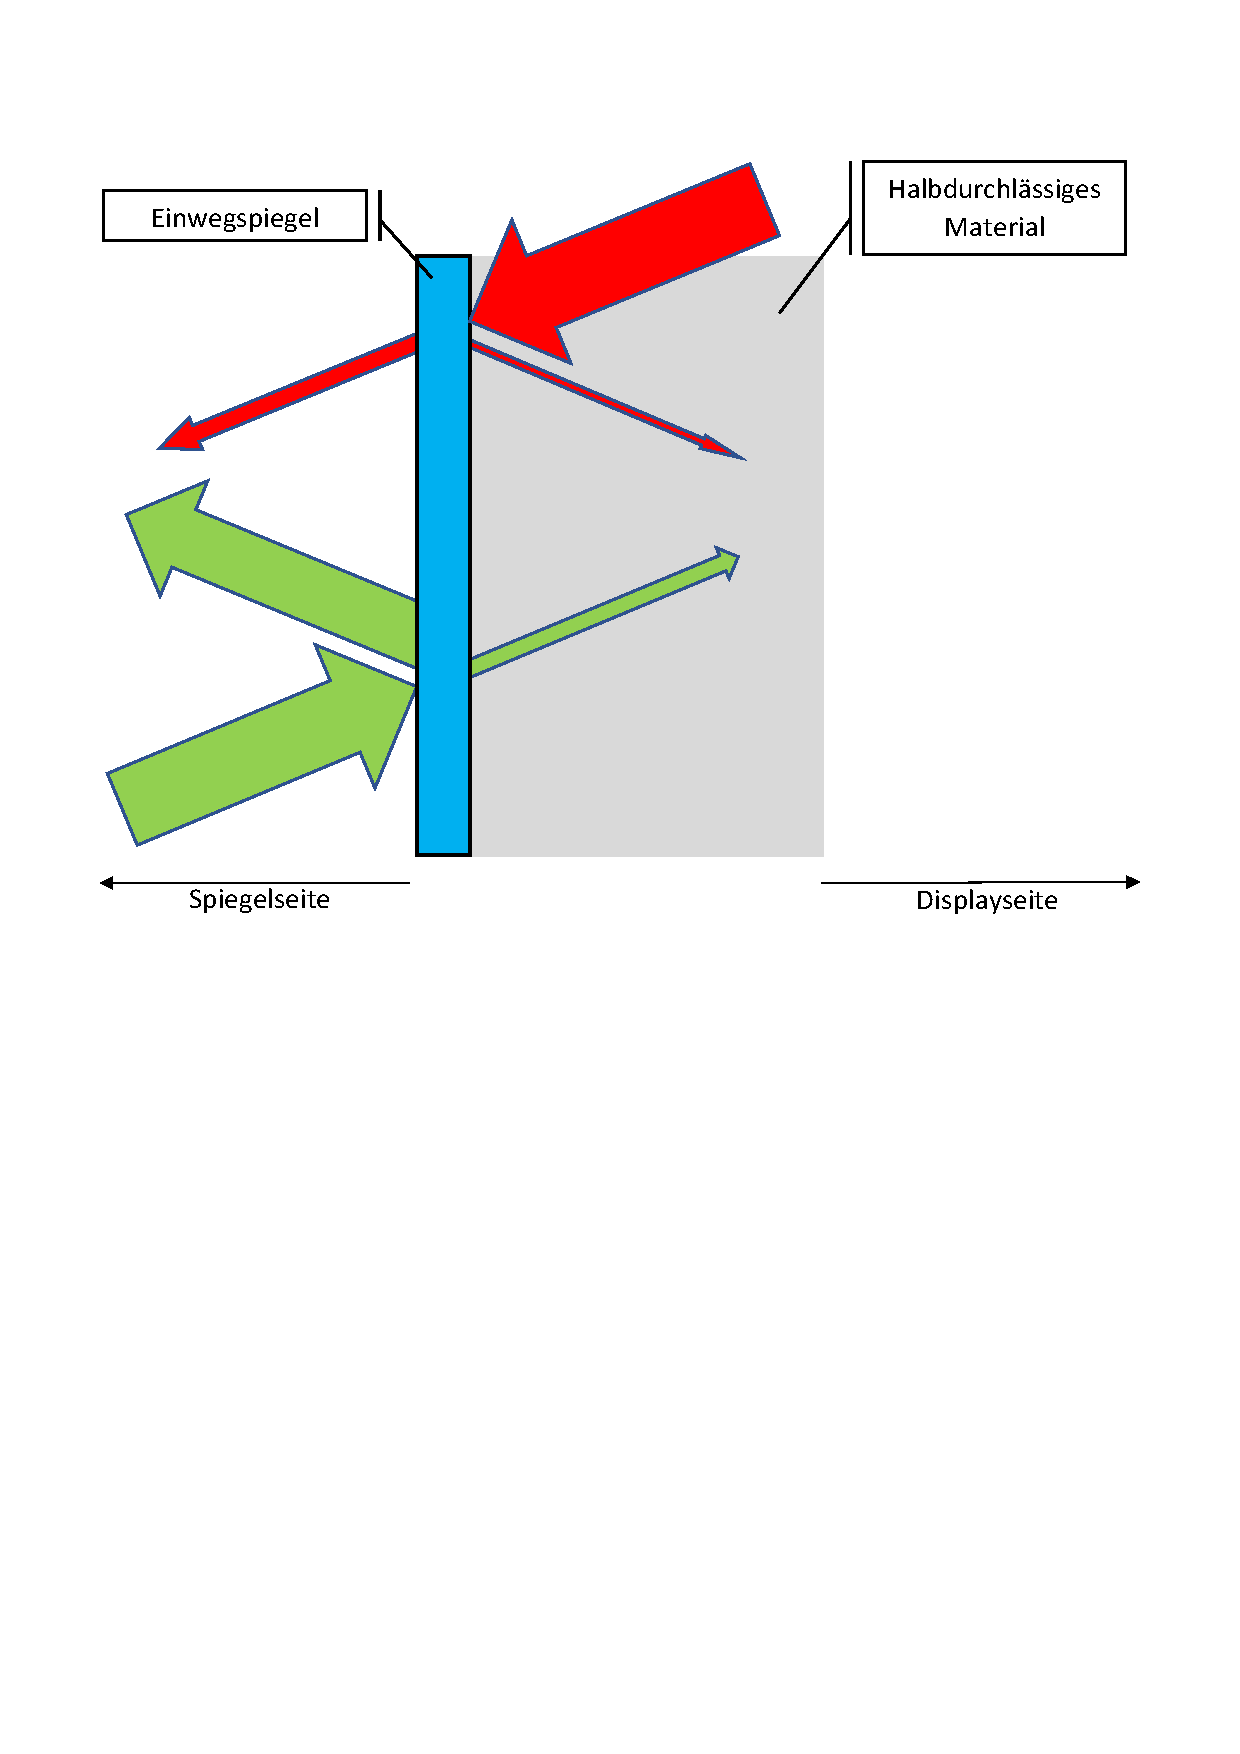
\includegraphics[trim=10mm 140mm 30mm 80mm, scale=0.35]{bilder/Einwegspiegel.pdf}
	\caption{Reflexions- und Transmissionswirkung}
	\label{fig:Spiegelfolie}
\end{wrapfigure}
Sie muss einerseits für den Spiegeleffekt reflektierend sein, gleichzeitig aber auch lichtdurchlässig (transmissiv) sein, damit die Anzeige des Bildschirms hindurch scheinen kann. 

Spiegel oder Folien mit diesen Eigenschaften heißen Spionspiegel (-folien) bzw. Einwegspiegel. Entscheidend für die Qualität der Anzeige ist das Verhältnis zwischen dem Reflexionsgrad und der Transmission (vgl. \autoref{fig:Spiegelfolie}). Der rote Pfeil in der Abbildung symbolisiert das Displaylicht und der grüne Pfeil das Umgebungslicht des Spiegels. Das Umgebungslicht wird zum größten Teil wieder reflektiert und das Displaylicht wird nahezu nach außen geleitet. Daher empfiehlt es sich einen Spiegel mit dem Reflexionsgrad von ca. 70-80\% und einem Transmissionswert von etwa 8\% zu verwenden. 


\subsubsection*{Folierung}
Die Folierung sollte in einem möglichst staubarmen Raum durchgeführt werden. Dabei wird 
ein Folienrakel oder eine Kreditkarte, eine Sprühflasche mit einer Wasser-Spülmittellösung (alternativ Scheibenreiniger), ein Cuttermesser und ein Scheibentuch bzw. Microfasertuch, was am besten keine Fuseln hinterlässt, als Hilfsmittel benötigt.
%\begin{figure}
%	\begin{center}
%		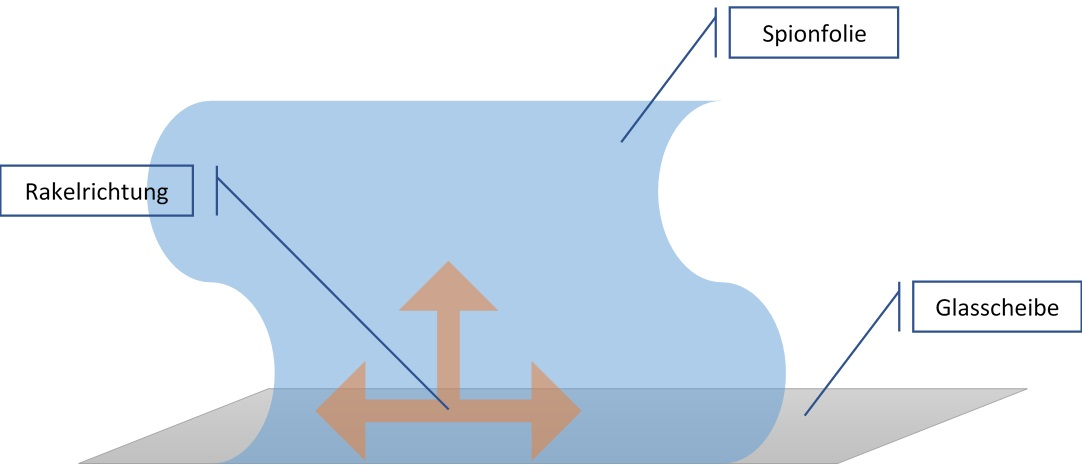
\includegraphics[scale=0.5]{bilder/Rakelanleitung.jpg}
%	\end{center}
%	\caption{Rakelrichtung}
%	\vspace{-10pt}
%\end{figure} 
Die Folie sollte idealerweise einige Zentimeter breiter und länger sein, als die Glasscheibe selbst, da Überstände im Nachgang mit dem Cuttermesser entfernt werden können. Die gründlich gereinigte Glasscheibe wird leicht mit dem Spülwasser befeuchtet, um eine Art Gleitschicht zu erzeugen. Nach Entfernung der Schutzschicht (falls vorhanden), wird die Folie auf die Glasscheibe aufgelegt. Vorhandene Luftbläschen werden mit Hilfe des Folienrakels heraus gestrichen (vgl. \autoref{fig:Folierung}). Ist das Ergebnis zufriedenstellend, sollte die Scheibe einen Tag liegen gelassen werden, bevor diese gereinigt und eingesetzt werden kann. Die Folierung erfordert selbst bei geringer Erfahrung nicht mehr als 15 Minuten. 

\begin{wrapfigure}{r}{0.45\textwidth}
		\includegraphics[scale=0.05]{bilder/spionspiegel.jpg}
		\caption{Folierung während des Proseminars}
		\label{fig:Folierung}
\end{wrapfigure}

Durch die Verwendung einer Spionspiegelfolie kann zwar eine akzeptable Qualität erzielt werden. Bessere Ergebnisse erfordern jedoch eine professionell beschichtete Glasscheibe wie beispielsweise von der Firma Glas Star aus Bochum, die sich auf die Herstellung von Glasscheiben für Smart Mirrors spezialisiert hat (vgl. \href{https://www.glas-star.de/spionspiegelnachmass/chrome-spy-spiegel/}{Link}). 	
	





\subsection{Monitor}
Um dem Benutzer alle gesammelten Daten anzeigen zulassen, wird ein Monitor benötigt. Der Monitor kann entweder als fertiges Produkt (mit oder ohne Gehäuse) eingebaut oder aus einem Display, einem Display Controller und einem Netzteil zusammengebaut werden. Im zweiten Fall ist die Kompatibilität der Komponenten zu berücksichtigen. Bei der Wahl des Displays sind neben den Kosten vor allem die Auflösung und die Stromversorgung entscheidend. Ebenfalls relevant ist der Schwarzwert des Displays, da ein hoher Schwarzwert für ein geringes Durchscheinen des Bildschirmhintergrundes sorgt. Zu empfehlen sind hier OLED Displays, die einen höheren Schwarzwert aufweisen als beispielsweise LCD Displays.  
\begin{figure}[H]
	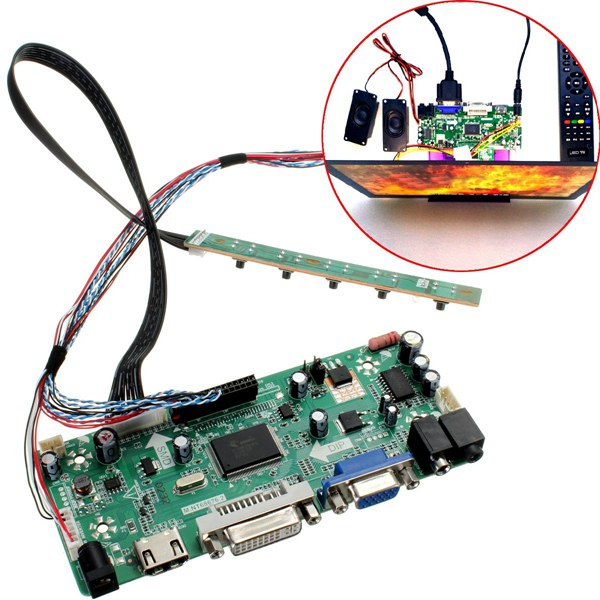
\includegraphics[trim=0mm 0mm 0mm 0mm, scale=1]{bilder/dcontroller.jpg}
	\caption{LCD Controller Board 40P}
	\label{fig:LCDController}
\end{figure}
Für das vorliegende Projekt wurde ein Acer V176Lbmd Monitor mit einer Diagonale von 17' (ohne Gehäuse)verwendet. Der Monitor ist mit einem DVI und VGA Anschluss ausgestattet. Der Display Controller wandelt das Ausgangssignal der Steuereinheit um und leitet die Informationen über einen 40 Pin LVDS Anschluss an das Display weiter (\autoref{fig:LCDController}). Der Display Controller besitzen lediglich einen VGA Anschluss, so dass bei einem HDMI Ausgang an der Steuereinheit ein HDMI zu VGA Adapter zur Übermittlung des Displaysignals benötigt wird.
 

\subsection{Steuereinheit und Sensoren}
Der \textit{SmartMirror} benötigt eine Steuereinheit zum Sammeln und Aufbereiten der anzuzeigenden Daten. Diese Daten werden alternativ über das Internet oder über Sensoren zusammen getragen. Neben einem Internetzugang werden somit auch Sensoren, konkret ein Bewegungssensor, sowie ein Temperatur- und Luftfeuchtigkeitssensor, benötigt.

\subsubsection*{Raspberry Pi 3}
\begin{figure}[H]
	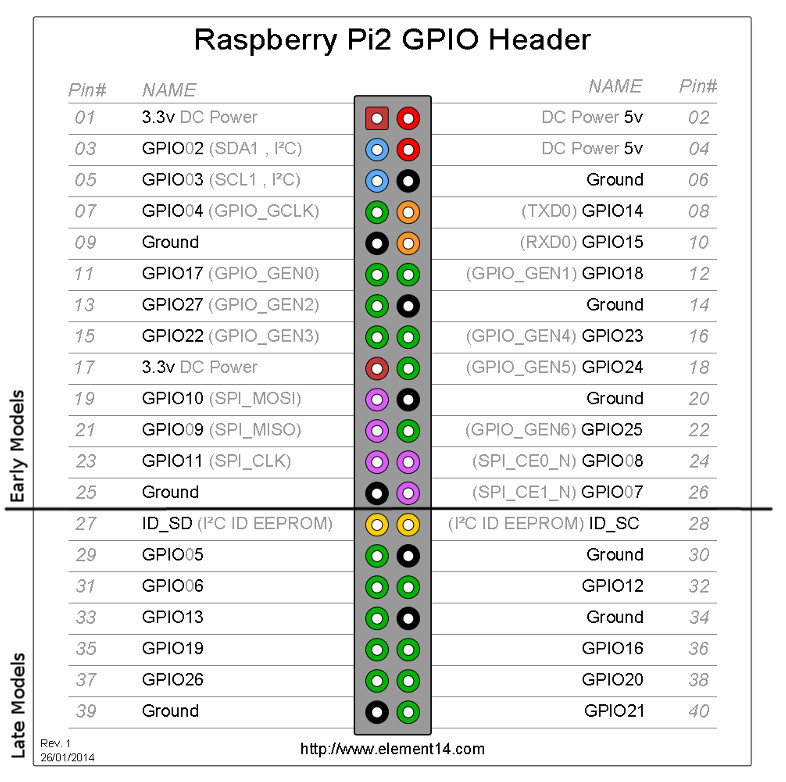
\includegraphics[scale=0.4]{bilder/gpio_pinout.jpg}
	\caption{GPIO-Belegung}
\end{figure}
Als Steuereinheit und Herzstück des \textit{SmartMirrors} dient ein Raspberry Pi 3 Model B. Das integrierte WLAN-Modul ermöglicht den mobilen Einsatz des \textit{SmartMirrors}, so dass dieser nicht fest an einen Ort gebunden ist. Für das Projekt werden lediglich einige der 40 GPIO-Anschlüsse des Boards für die Sensoren benötigt. Die genau Belegung der GPIO-Anschlüsse ist in Abbildung 5 grafisch dargestellt.

Unter dem Link \url{https://www.raspberrypi.org/documentation/} ist eine ausführliche Dokumentation zu den Eigenschaften des Raspberry Pi zu finden. Da der Raspberry Pi üblicherweise ohne ein Betriebssystem geliefert wird, wird unter der bereits genannten Adresse ebenfalls eine detaillierte Betriebssystem-Installationsanleitung bereit gestellt. Für das Projekt wird als Betriebssystem die ,,RASPBIAN JESSIE WITH DESKTOP`` Distribution verwendet. Alternativ zur Desktop Version gibt es auch eine Light Version. Diese ist wegen der fehlenden grafischen Oberfläche für dieses Projekt ungeeignet.

\subsubsection*{Bewegungssensor}
Der Bewegungssensor wird eingesetzt, um je nach Bedarf das Display ein- und auszuschalten und somit Energie zu sparen. Betritt eine Person den Raum, indem der Spiegel hängt, soll  der Sensor ein Signal zum Einschalten des Displays geben. Andernfalls bleibt das Display ausgeschaltet. 

	\begin{wrapfigure}{l}{0.4\textwidth}
		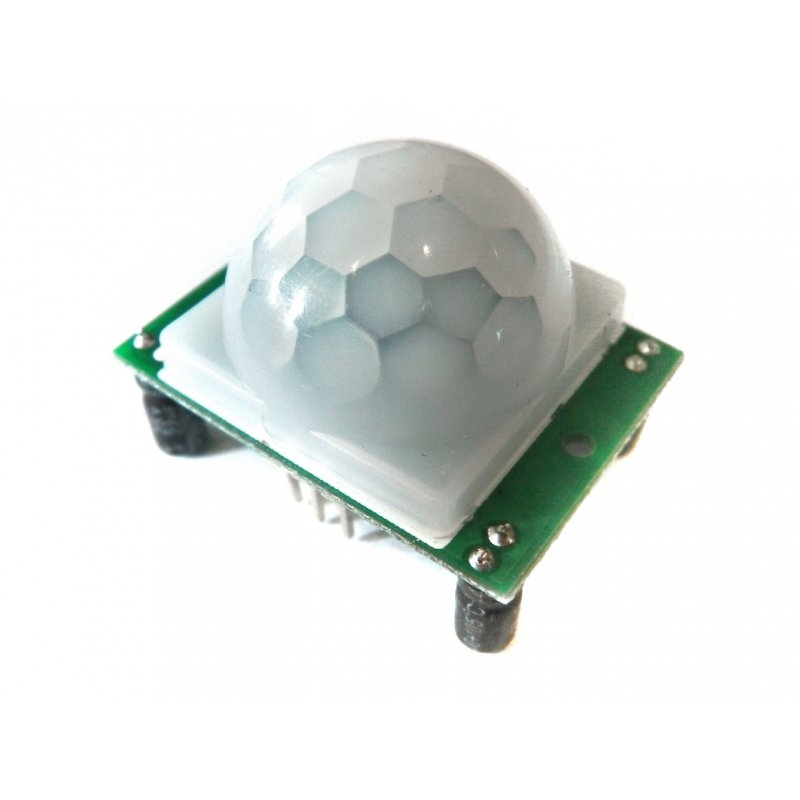
\includegraphics[width=0.9\textwidth]{bilder/PIR-Sensor.jpg}
		\caption{PIR-Sensor HC-SR501}
	\end{wrapfigure}	
Als Bewegungssensor für diesen Zweck ist das Modell HC-SR501 sehr gut geeignet. Der PIR-Sensor oder auch ,,IR-Bewegungssensor`` arbeitet passiv auf Basis der Infrarotstrahlung der Umgebung. Jeder Körper sendet eine kleine Menge an Infrarotstrahlung aus. Der PIR-Sensor stellt die Temperaturänderung im Raum fest und kann somit als Schalter verwendet werden. Der Sensor befindet sich auf einer kleinen Platine, besitzt eine einstellbare Empfindlichkeit und zwei M2 Befestigungsbohrungen für die Montage. Die Reichweite der Erfassung beträgt bis zu 7 Meter. Der Erfassungswinkel des Objektives beträgt etwa 100 Grad. 

Zum Anschließen des Sensors an den Raspberry Pi 3 werden zusätzlich drei Jumperkabel benötigt (VCC an Pin2 (5V); OUT an Pin16 (GPIO 23); GND an Pin6 (Ground)). Alternativ dazu kann ein dreiadriges Kabel verwendet werden.

\subsubsection*{Temperatur- und Luftfeuchtigkeitssensor}
Der Temperatur- und Luftfeuchtigkeitssensor liefert Daten über den Raum, in dem der Spiegel hängt. Dazu ist der Sensor lediglich an das Raspberry Pi Board anzuschließen.
%\begin{figure}[H]
%	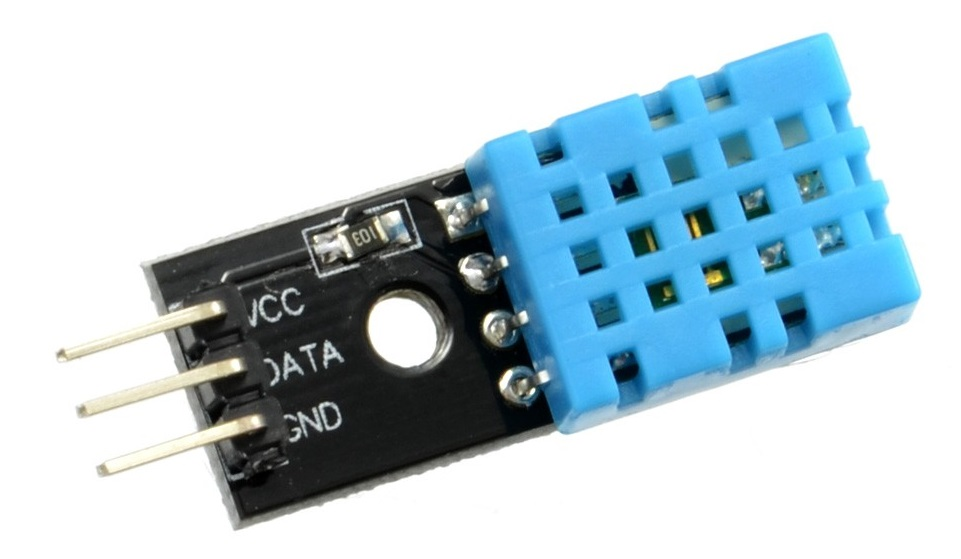
\includegraphics[trim=0mm 0mm 0mm 0mm, scale=0.3]{bilder/DHT11.jpg}
%	\caption{TL-Sensor DHT11}
%\end{figure}
 Der linke Pin (VCC) des Sensors wird an den Pin1 (3.3V) des Pi´s angeschlossen. Der mittlere Sensor Pin (DATA)  ermöglicht den Datenaustausch und wird mit einen freien GPIO Pin des Raspberry Pi´s (z.B. Pin7) verbunden. 
\begin{figure}[H]
	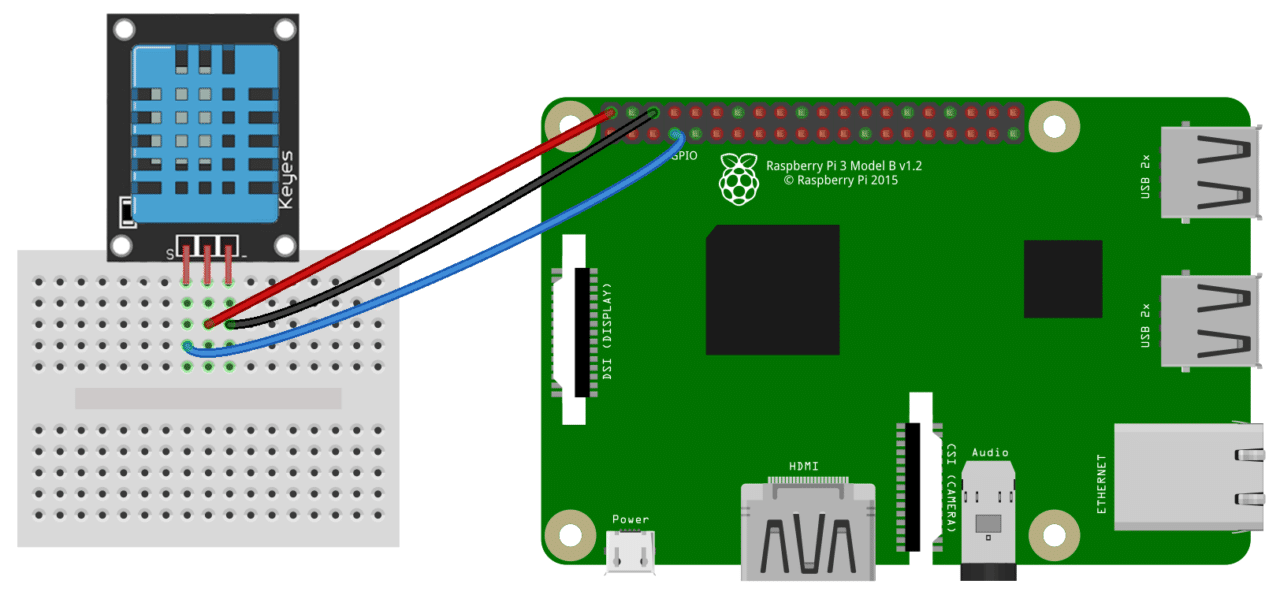
\includegraphics[trim=0mm 0mm 0mm 0mm, scale=1]{bilder/DHT11-on-the-Raspberry-Pi.png}
	\caption{DHT11 angeschlossen an ein Raspberry Pi}
\end{figure}
Der rechte Sensor Pin (GND) muss mit einem der Ground Pin´s (z.B. Pin5) des Raspberry Pi´s verbunden werden. Die Abbildung 8 illustriert den Anschluss des Sensors an ein Raspberry Pi bei Verwendung einer Steckplatine. Anzumerken ist, dass der linke und mittlere Anschluss in der Abbildung vertauscht sind.

\subsection{Aufbau}
Die \autoref{fig:Skizze} zeigt einen Überblick über die Anordnung und Platzierung der verbauten Komponenten. 
\begin{figure}
	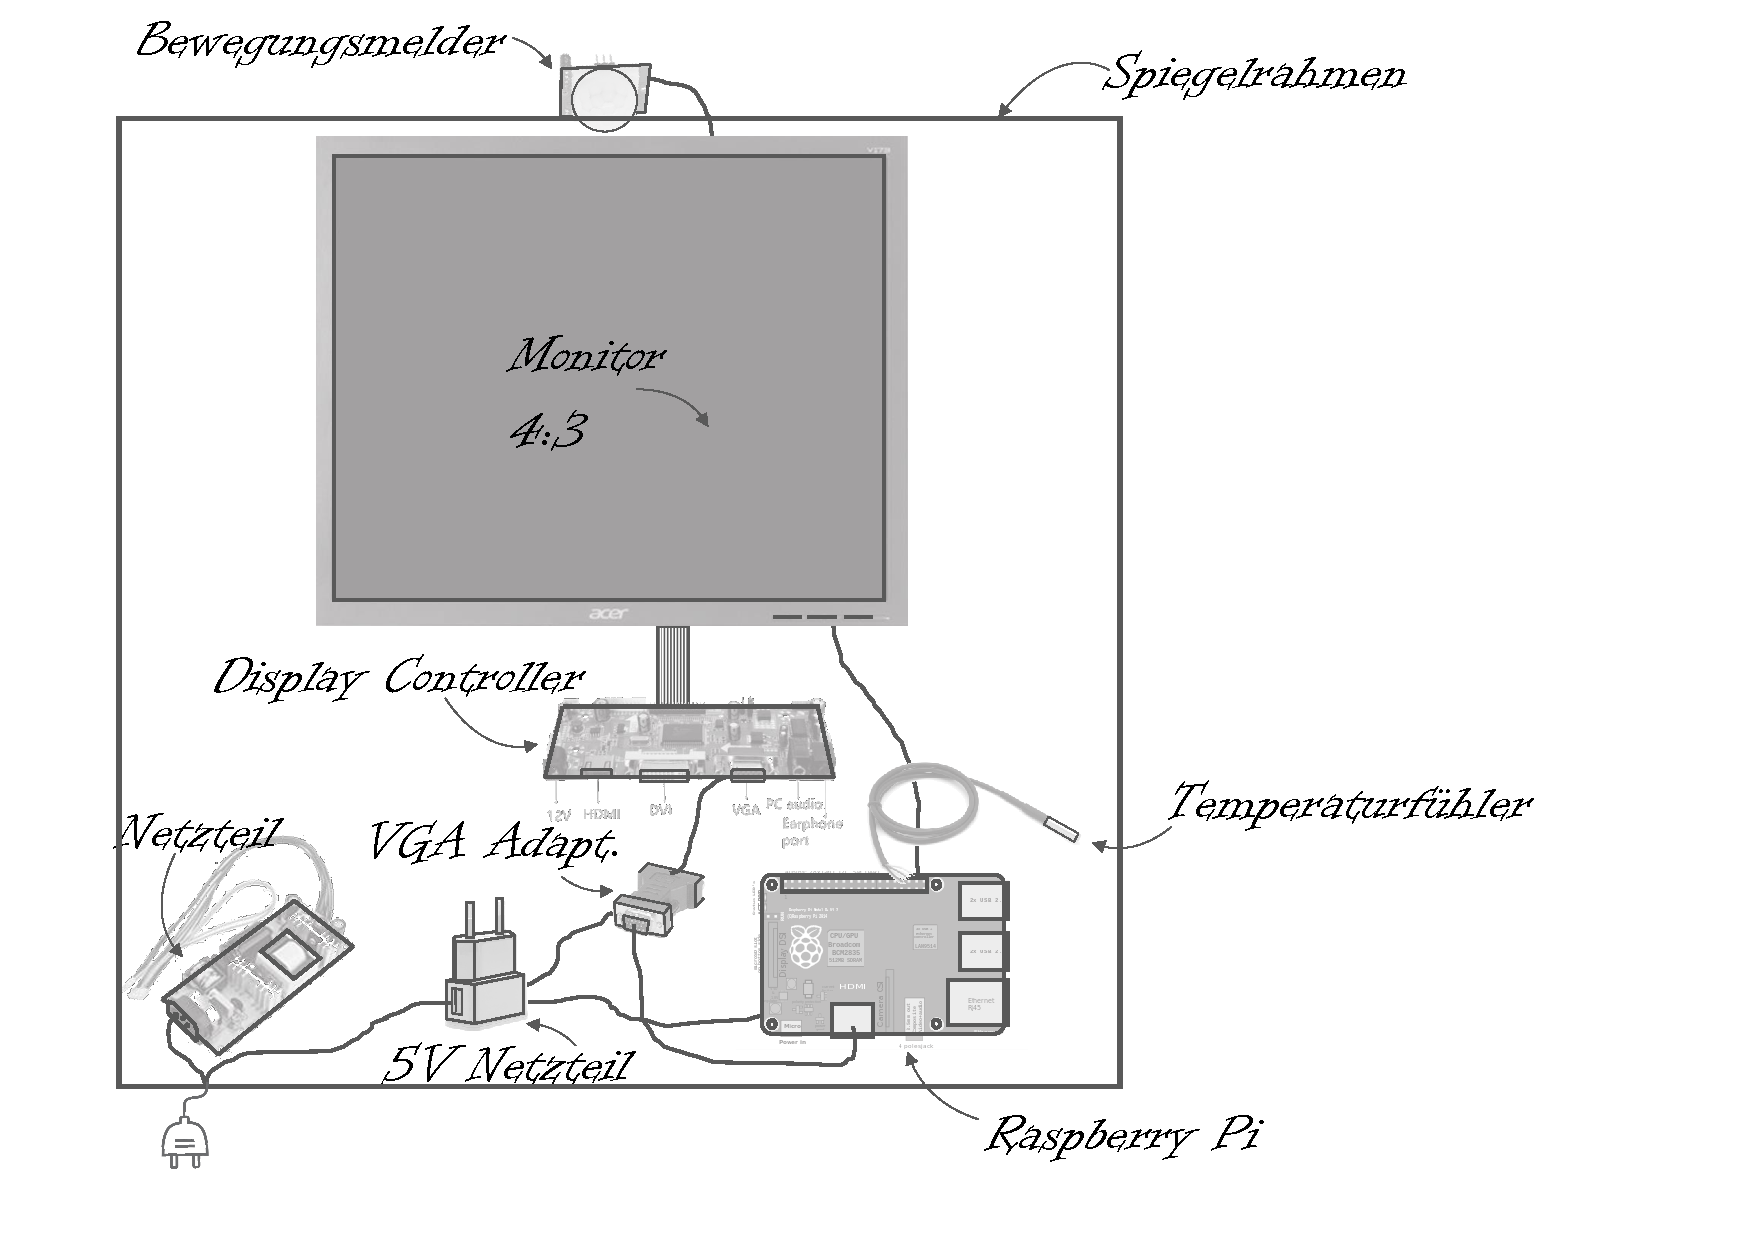
\includegraphics[scale=0.5, trim=0mm 10mm 60mm 10mm]{bilder/smartMirrorExplosionsskizze.pdf}
	\caption{Konstruktionsskizze}
	\label{fig:Skizze}
\end{figure}
Da der Monitor den meisten Platz erfordert, müssen die übrigen Komponenten um das Display herum untergebracht werden. Es ist zu berücksichtigen, dass der Monitor mit  minimalem Abstand zur oberen Kante des Rahmens verbaut wird, damit der Spiegel je nach Form nicht zu weit nach oben gehangen werden muss. Zur Verbesserung des Halts der Komponenten, wird eine Hartschaumplatte eingesetzt. 

\begin{wrapfigure}{r}{0.45\textwidth}
	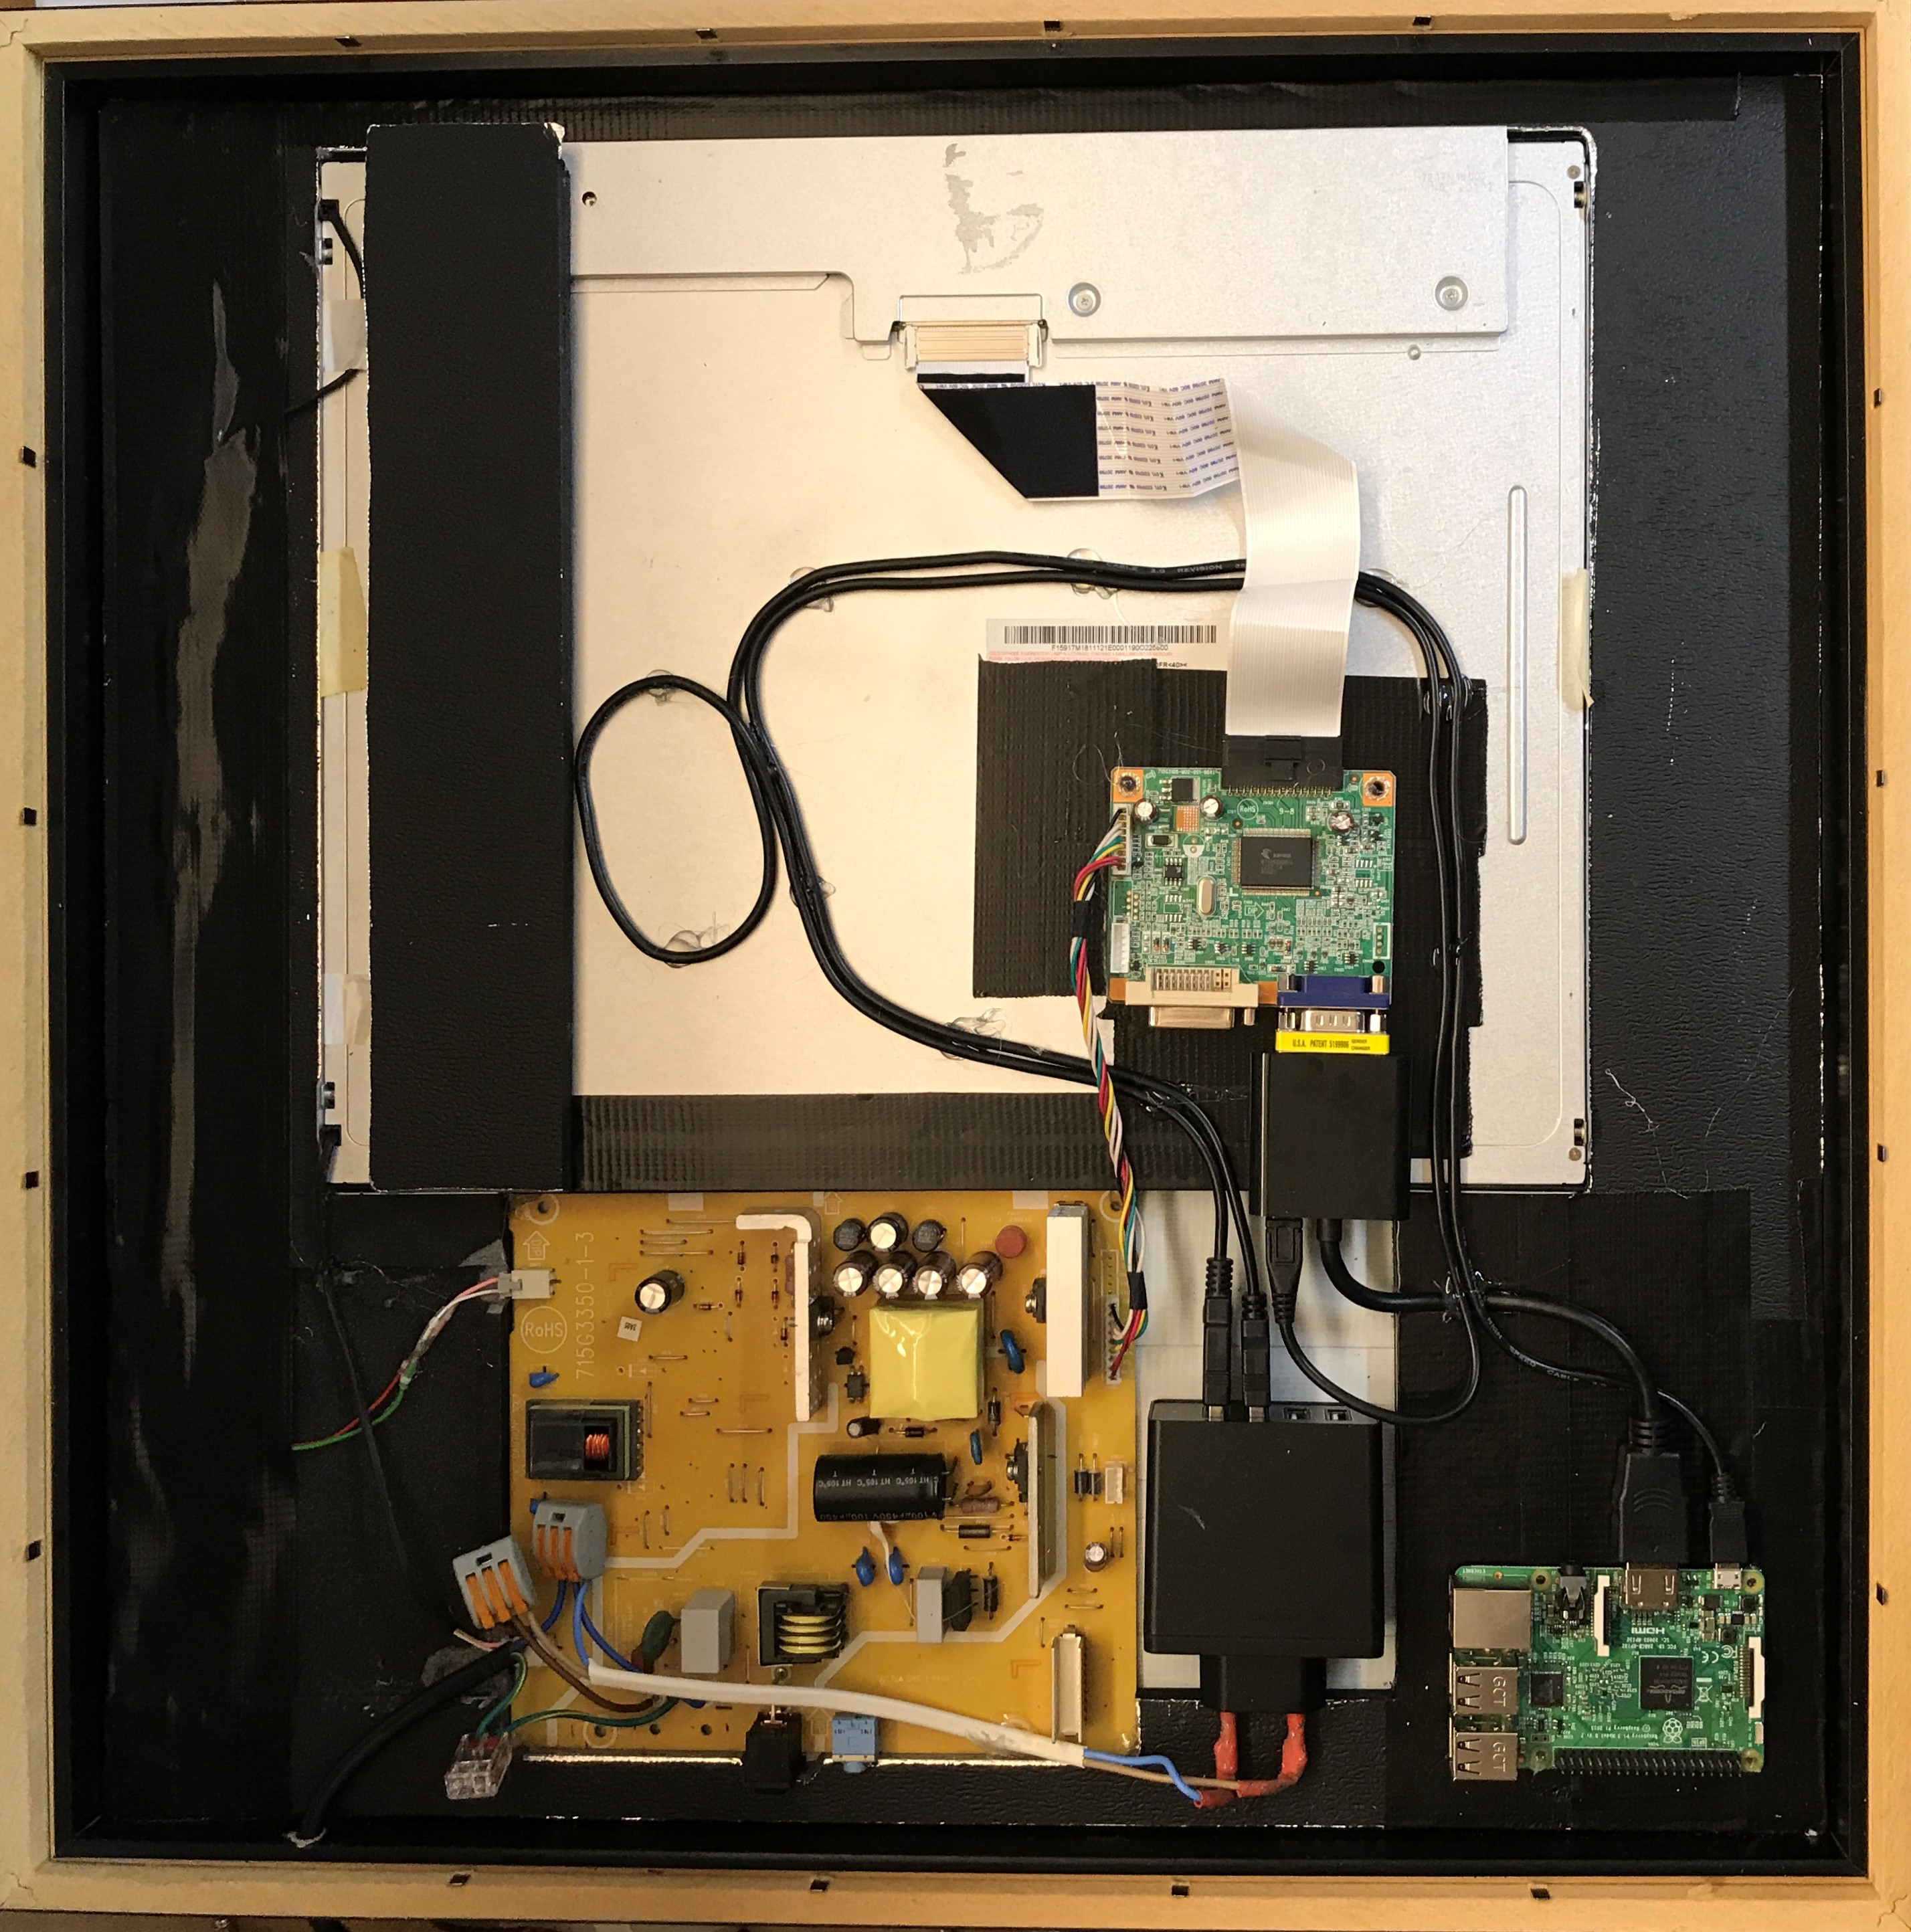
\includegraphics[scale=0.06]{bilder/Innenansicht.jpg}
	\caption{Anordnung und Verkabelung der Komponenten}
	\label{fig:Innenansicht}
\end{wrapfigure}
Dazu wird ein Loch passend zur Größe des Displays ausgeschnitten und die anderen Komponenten auf der Platte platziert. Die Hartschaumplatte und die Rückwand sind für ein besseres Ergebnis des Spionspiegels von innen schwarz lackiert (Abbildung 12-13). 
Die dunkle Farbe absorbiert das eintretende Licht und vermindert die Reflexion. Ein Abbild der Rückseite wird in \autoref{fig:Innenansicht} repräsentiert.

%\begin{figure}[H]
%	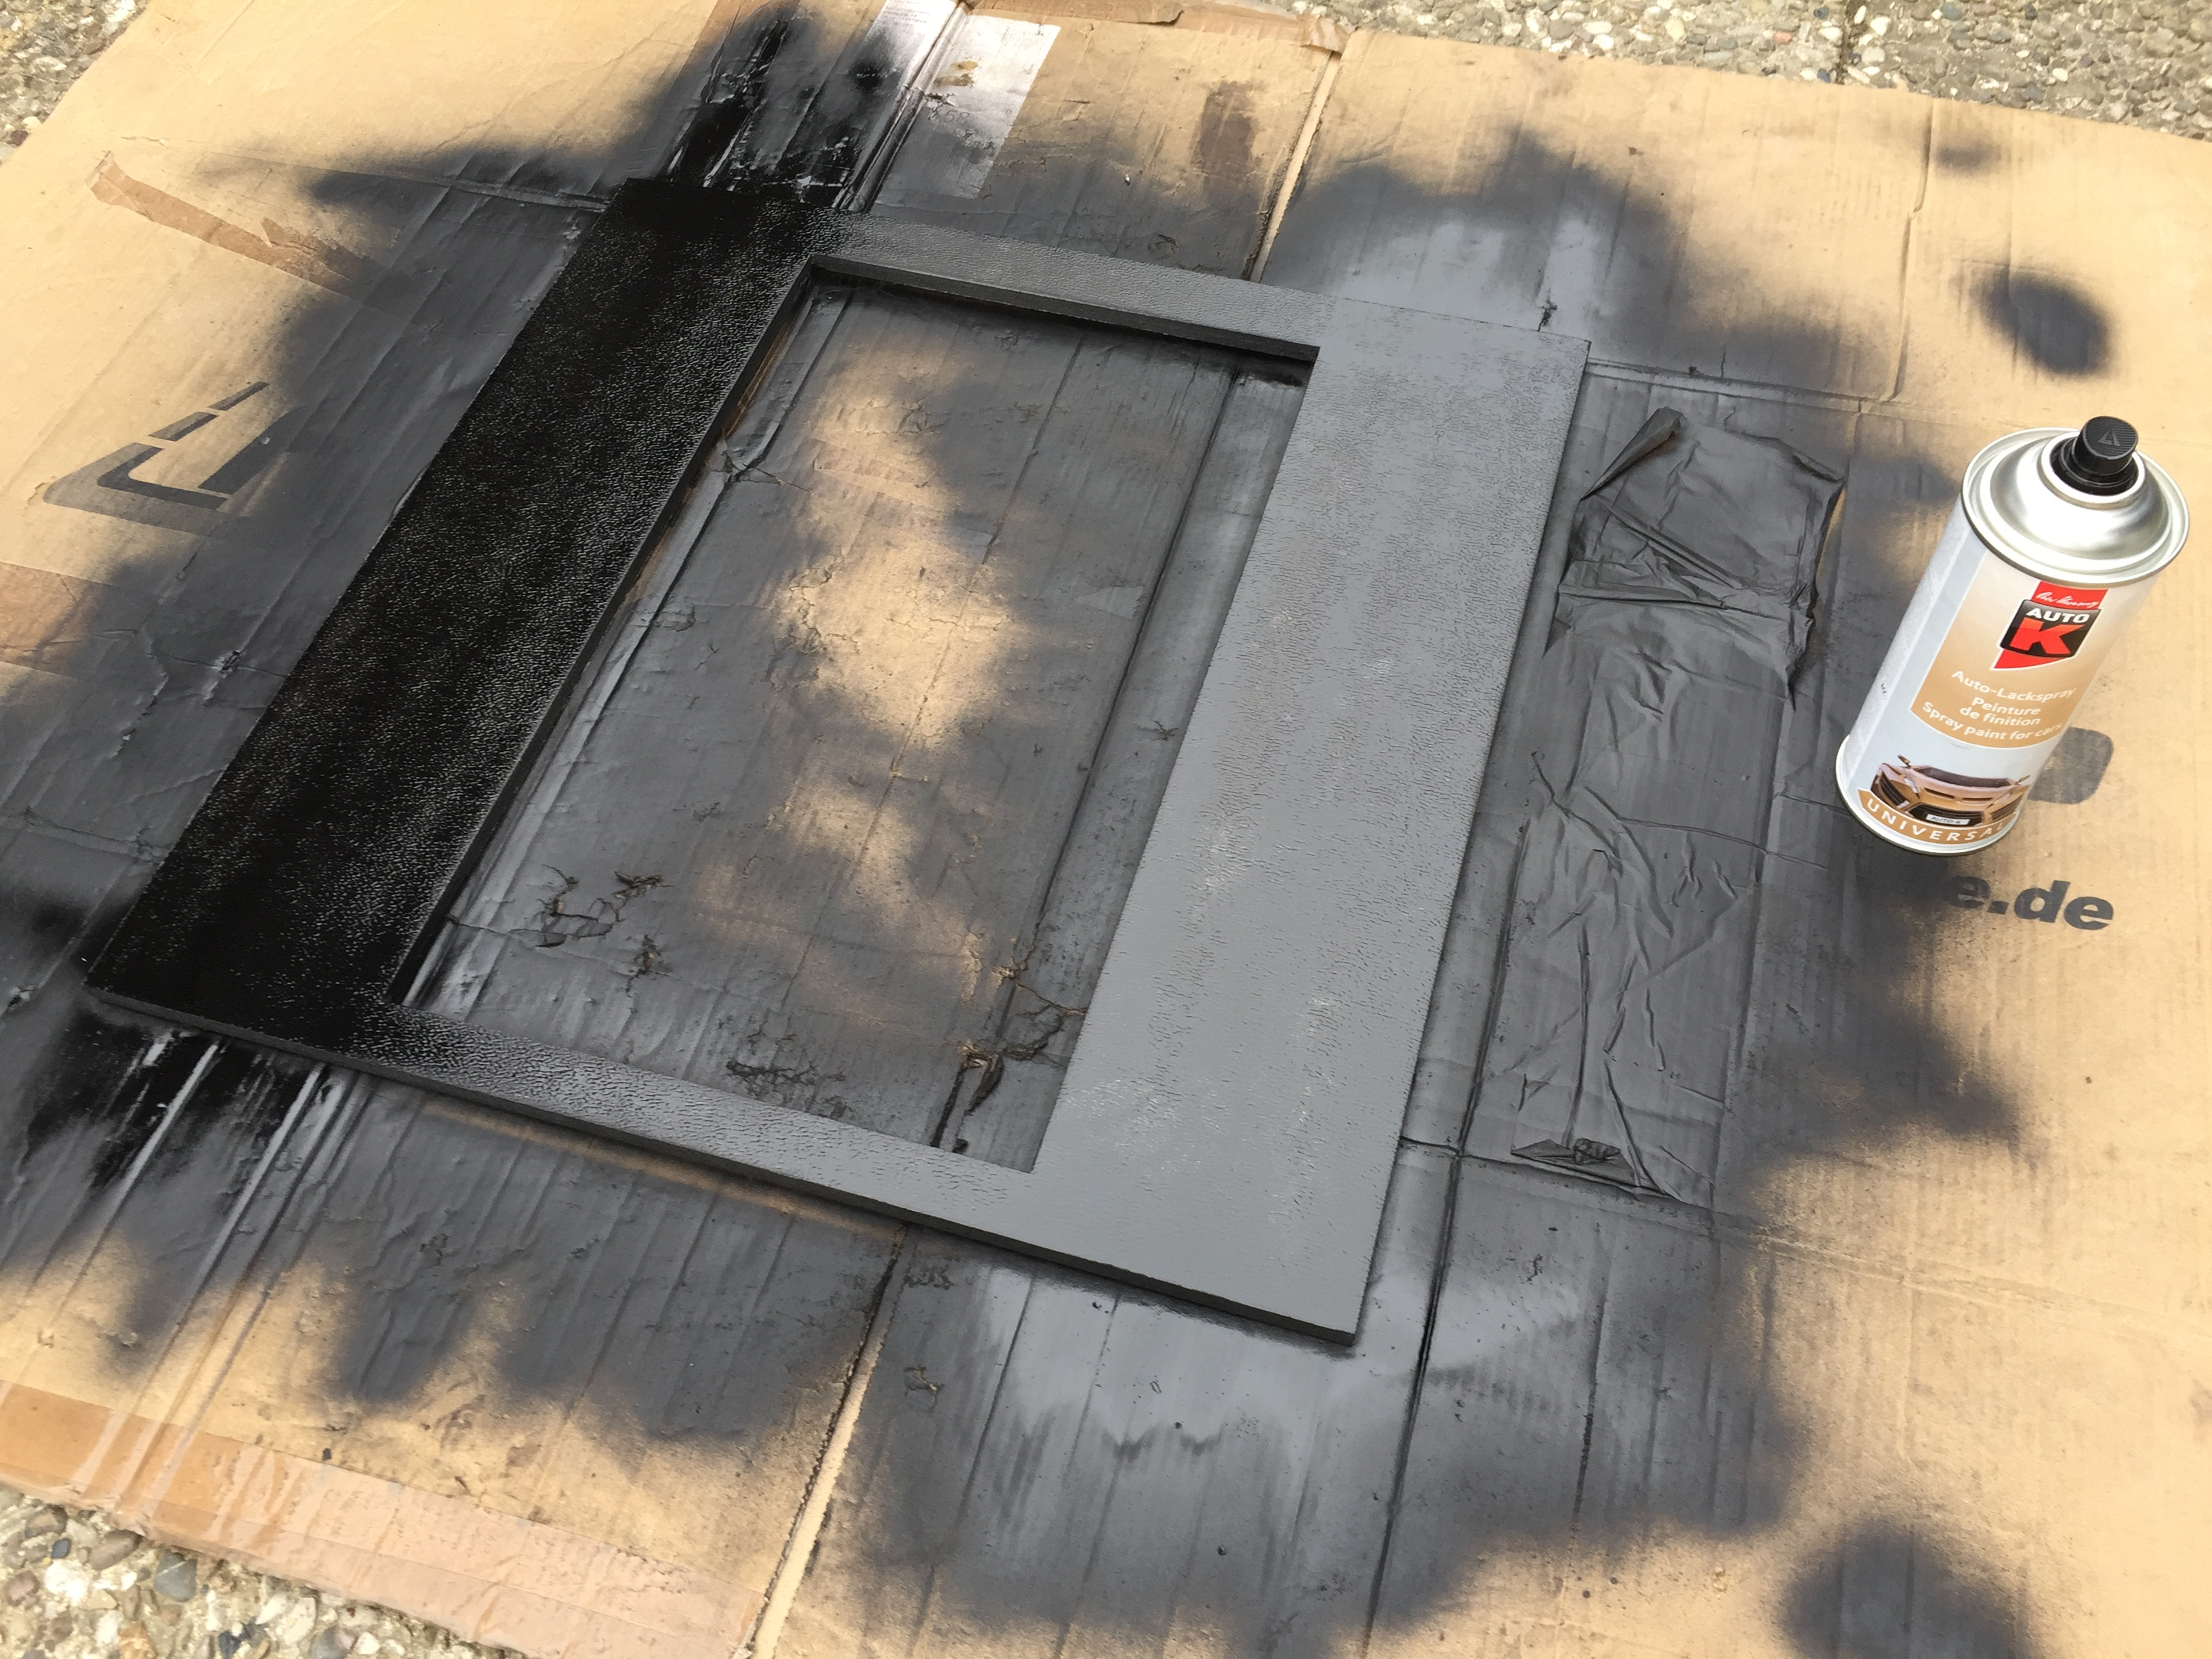
\includegraphics[scale=0.06]{bilder/Hartschaumplatte.jpg}
%	\caption{Lackierung der Hartschaumplatte}
%\end{figure}
%\begin{figure}[H]
%	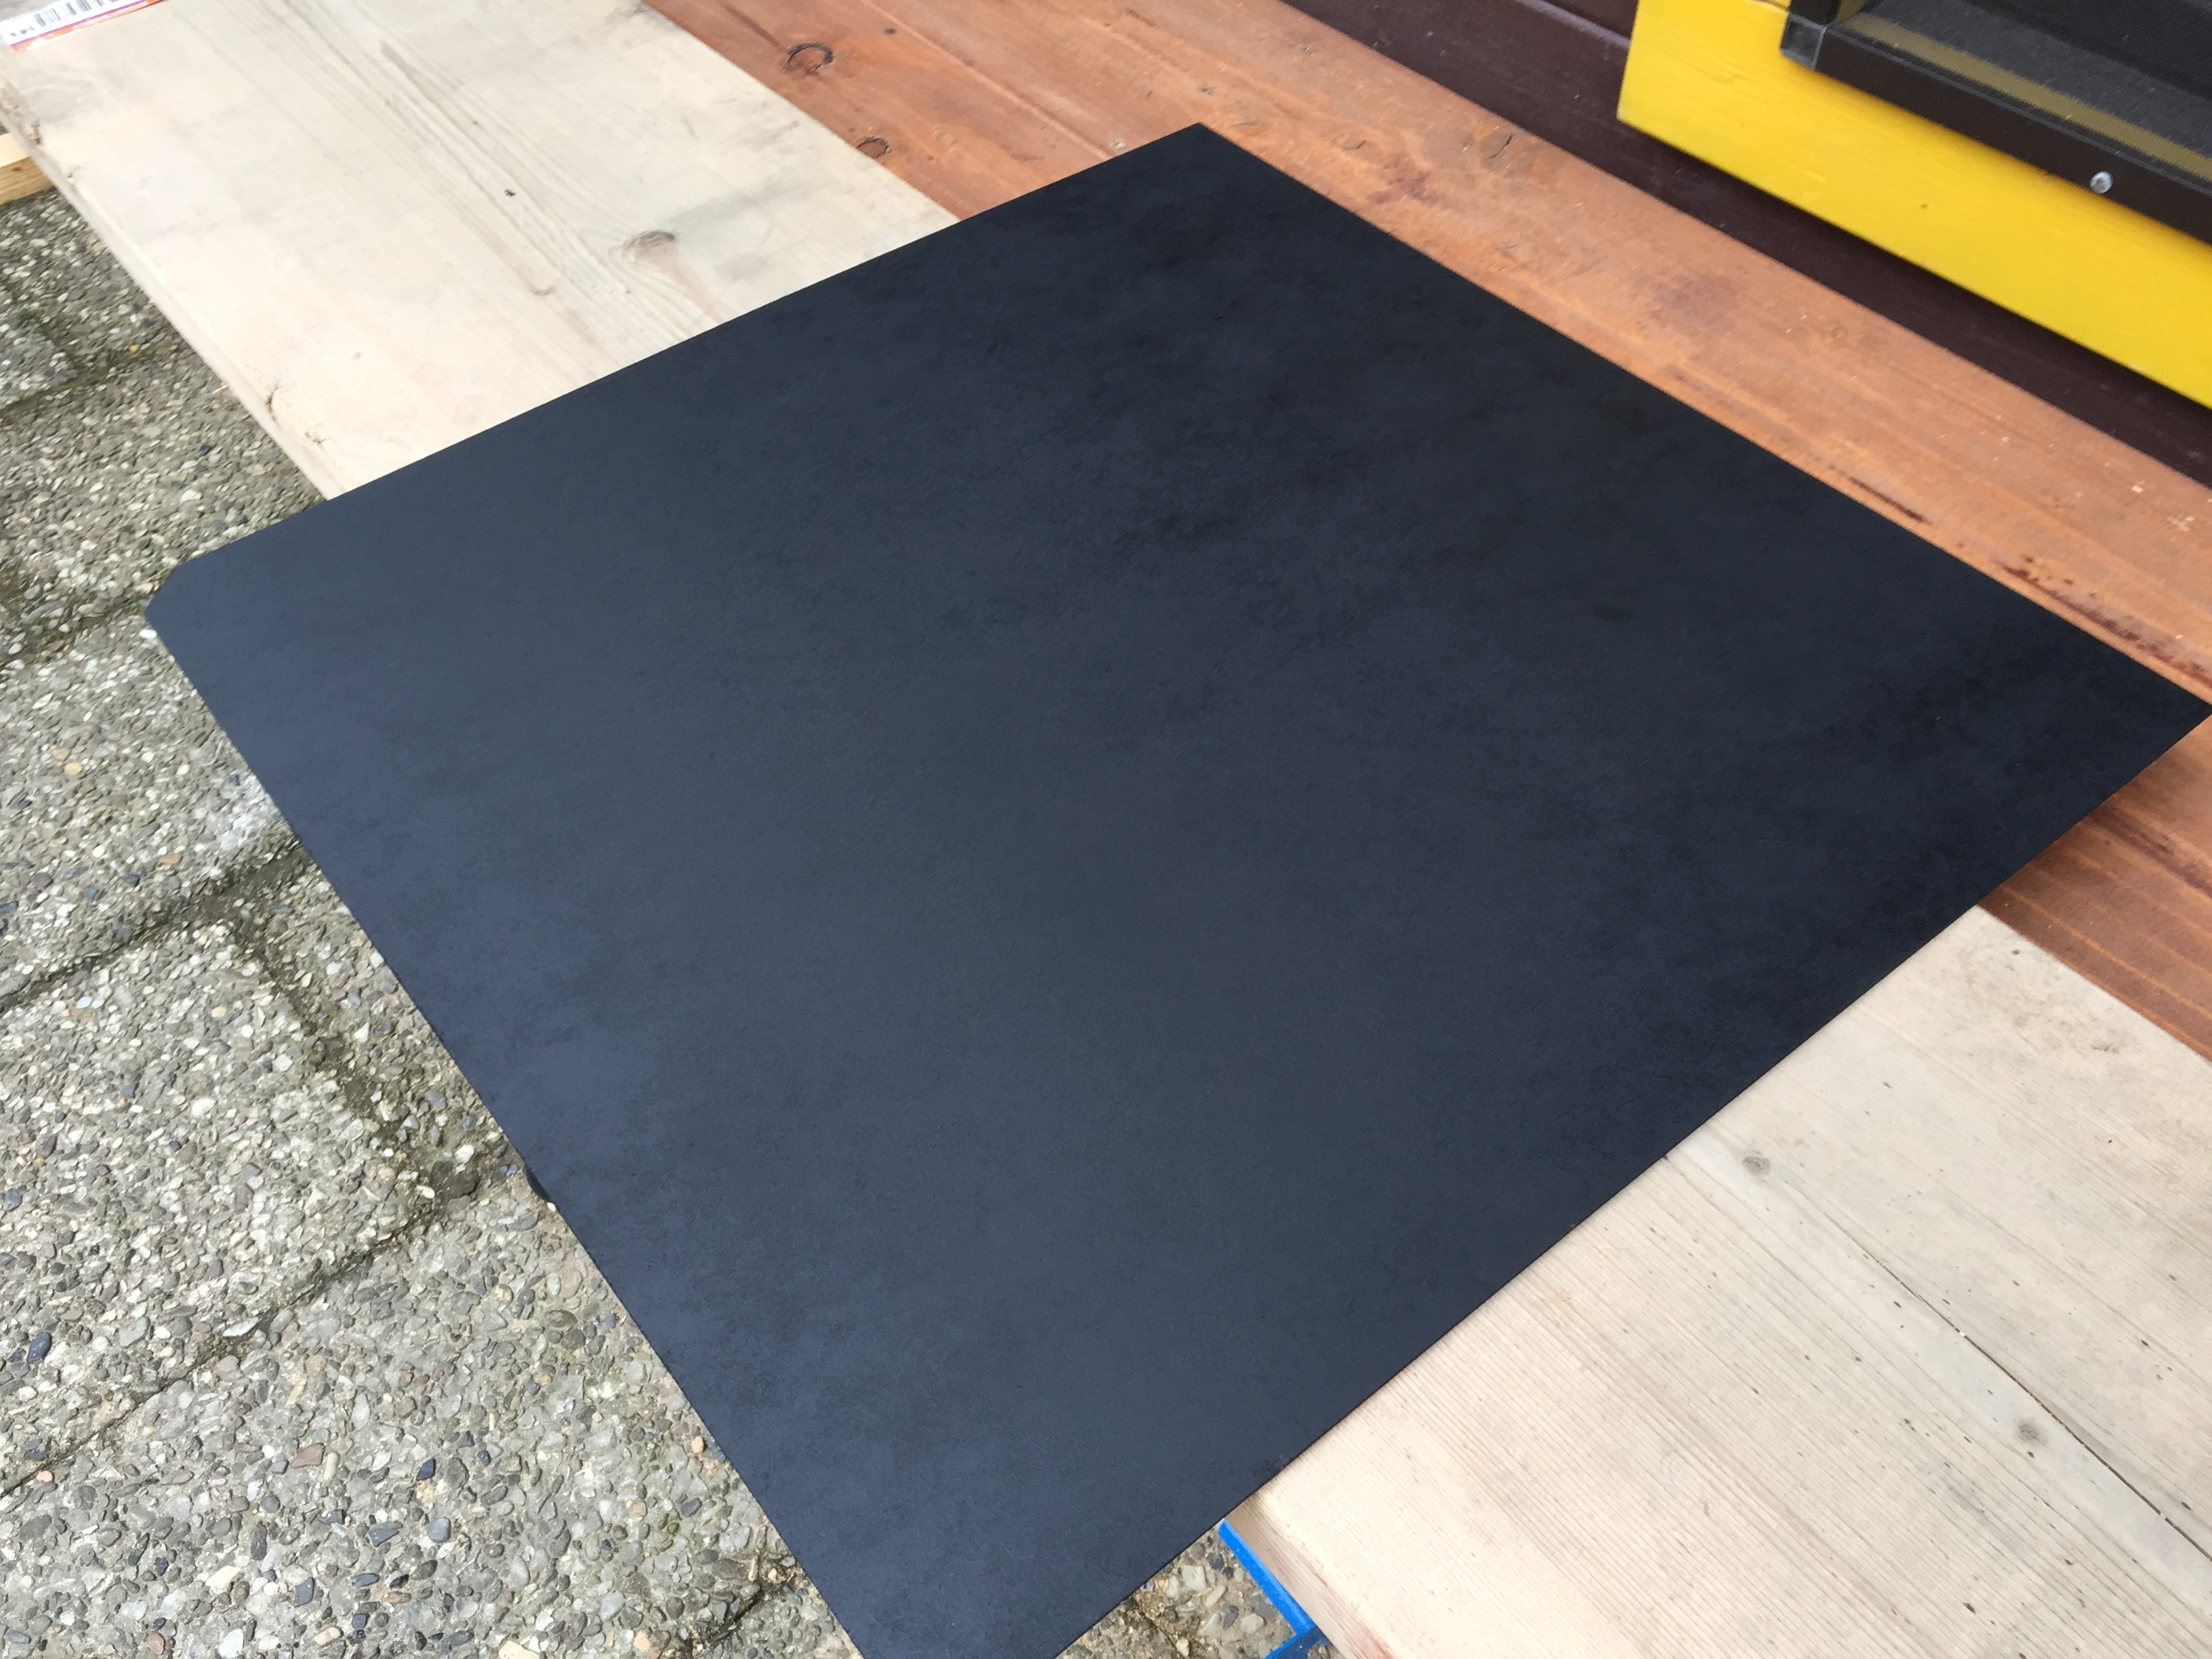
\includegraphics[scale=0.06]{bilder/Rueckwand.jpg}
%	\caption{Lackierung der Rückwand}
%\end{figure}

% kapitel2.tex
%\chapter{Die Softwarekonstruktion}
%\label{chapter:kap2}
\section{Aufbau der Softwarearchitektur}
Wie im ersten Teil der Ausarbeitung verdeutlicht wurde, ist der Raspberry Pi im Inneren des Spiegels das Kernstück der gesamten Plattform. Auf dieser Hardwarekomponente läuft dementsprechend die komplett entwickelte Software. 

Das Softwareprojekt selbst ist in zwei Komponenten aufgeteilt. Die erste Softwarekomponente realisiert die eigentliche SmartMirror-Anwendung inklusive der Ausgestaltung der Benutzungsschnittstelle, der Kommunikation mit verbauten Sensoren und des Datenimportes aus Datenquellen des Internets. Diese Anwendung ist in Python geschrieben, realisiert die SmartMirror-Funktionalität und hat den größten Anteil des Implementierungsaufwandes erfordert. Im Gegensatz dazu steht die zweite Softwarekomponente, im folgenden StartUp-Anwendung genannt, die ein Skript umfasst, das nach dem Systemstart die SmartMirror-Anwendung startet. Bei dieser handelt es sich eher um eine erforderliche Hilfskomponente von geringerem Umfang, die als Bash-Skript direkt ausführbar auf Betriebssystemebene realisiert wurde.  

\begin{figure}
	\centering
	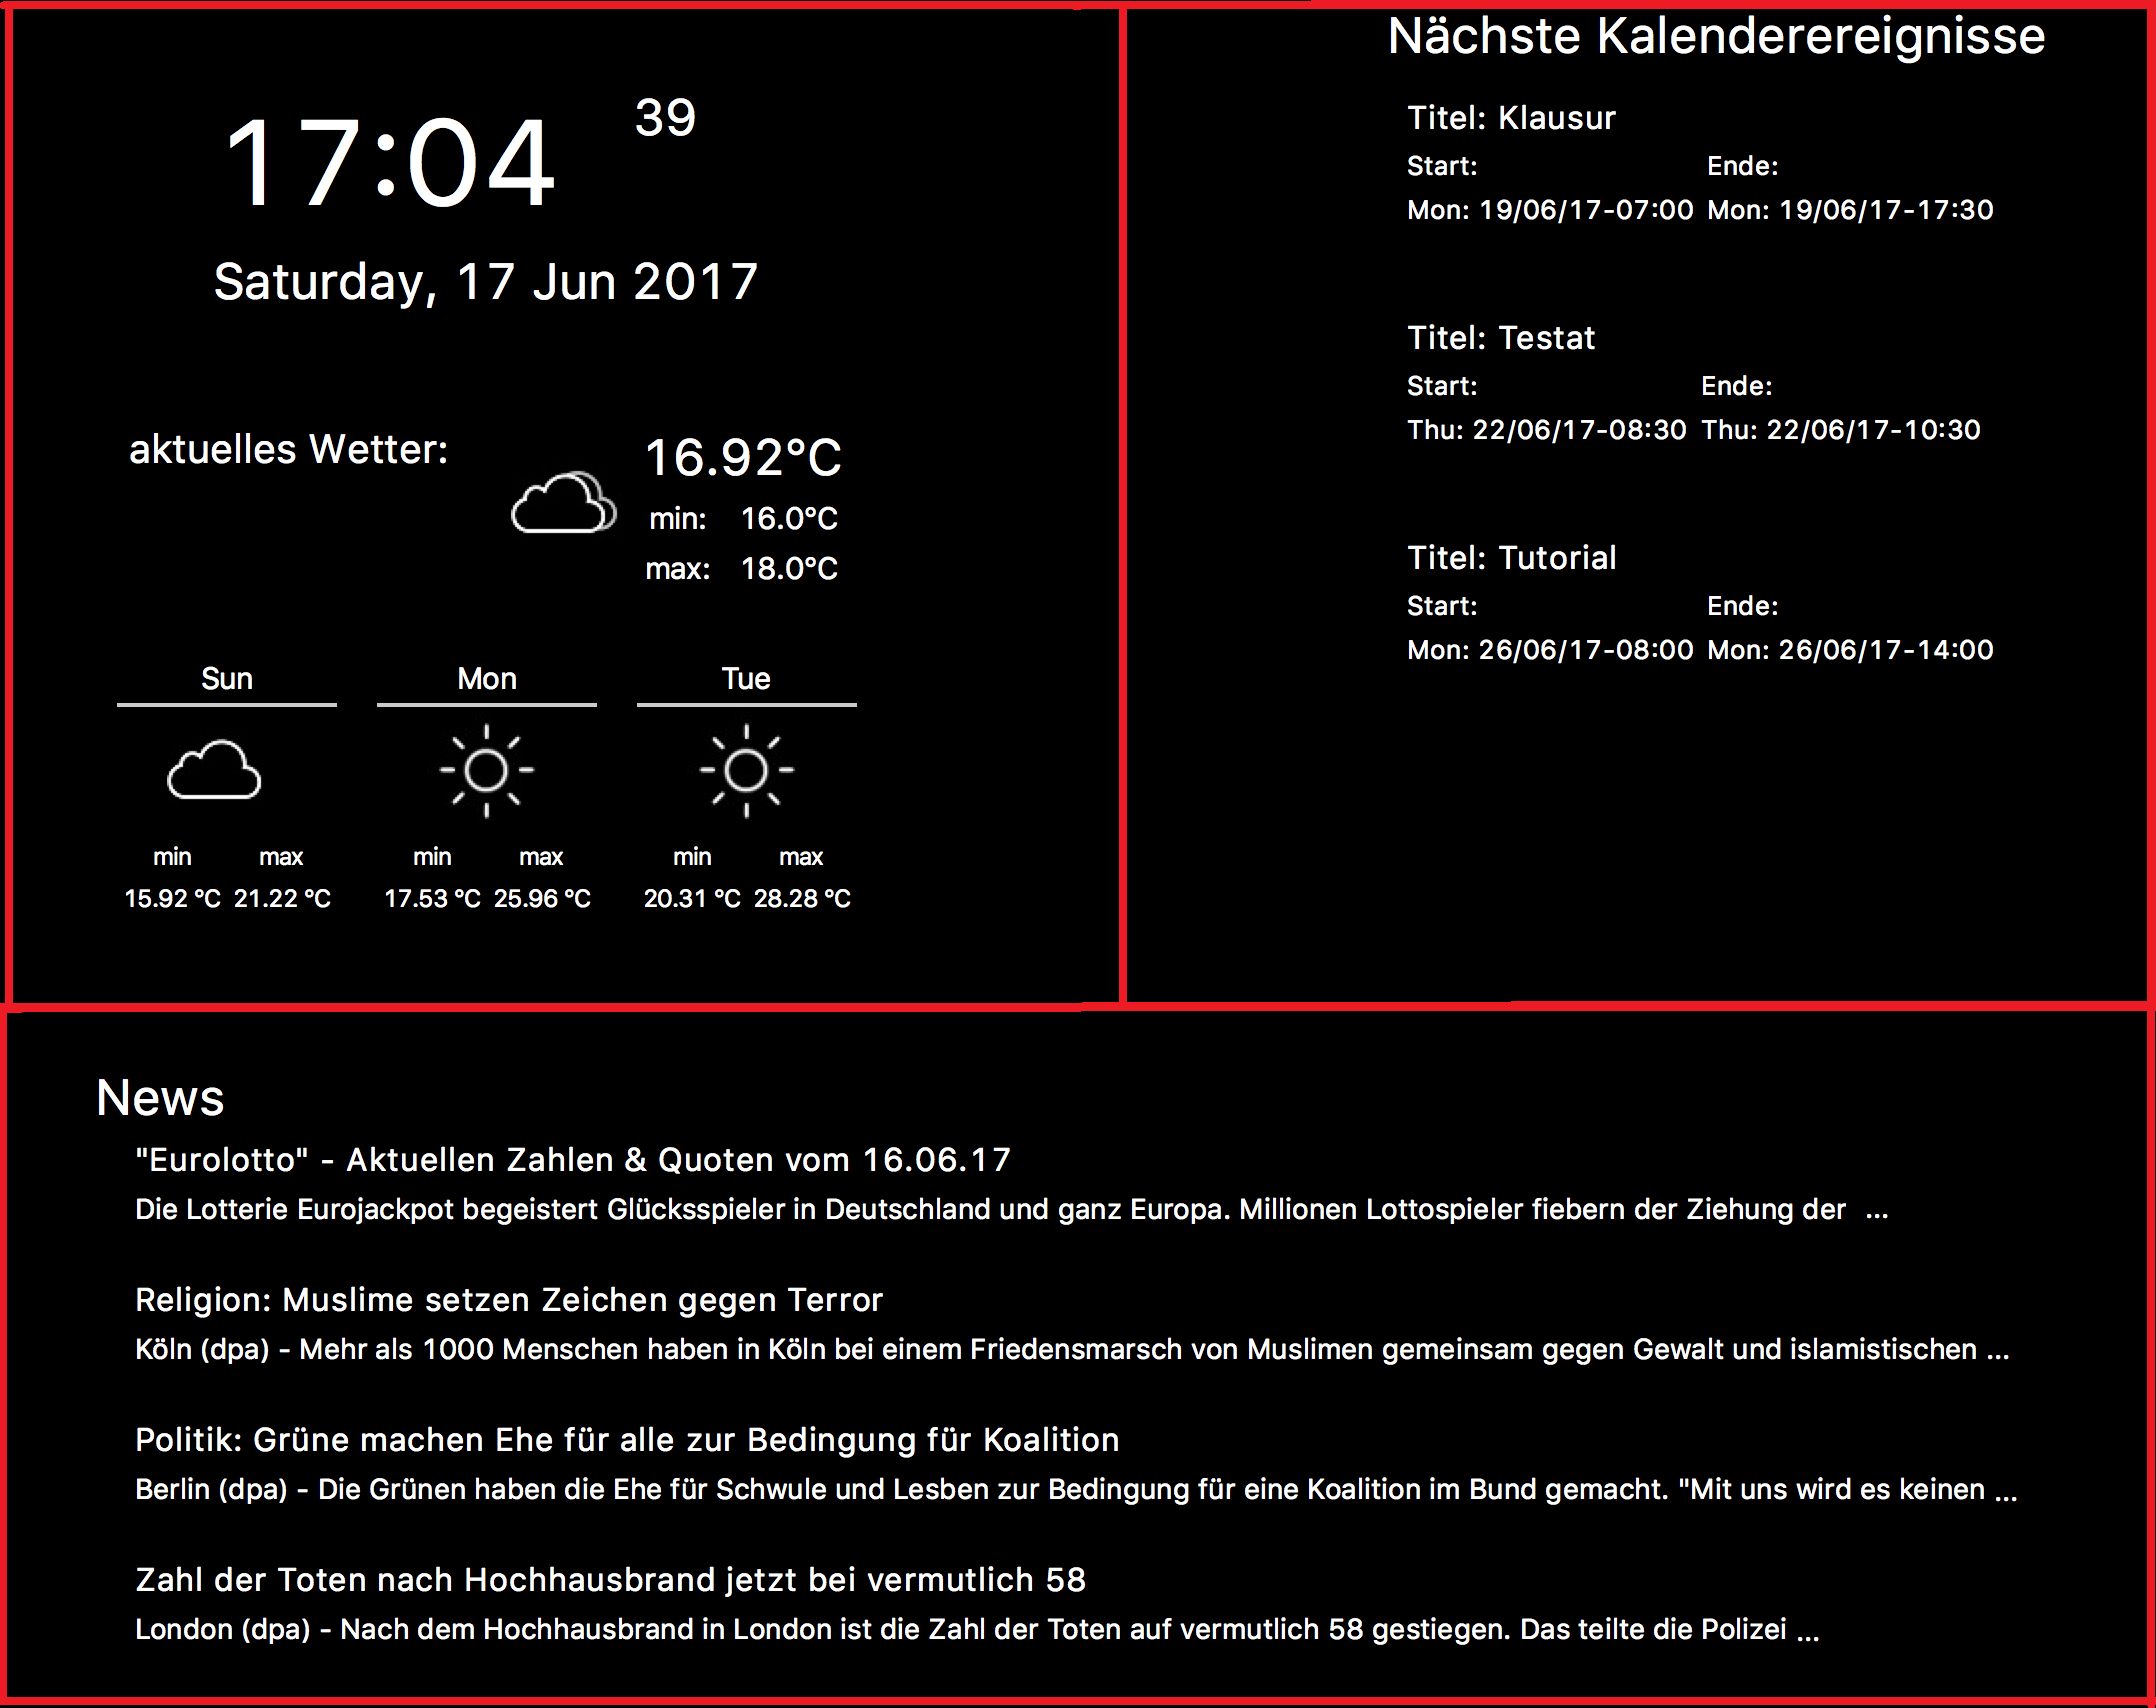
\includegraphics[width=0.7\linewidth]{bilder/grafOberflaeche}
	\caption[Verteilungsdiagramm der SmartMirror-Applikationen]{Verteilungsdiagramm der SmartMirror-Applikationen}
	\label{fig:verteilungsdiagramm}
\end{figure}

Zum besseren Verständnis ist in \autoref{fig:verteilungsdiagramm} der softwaretechnische Technologiestack der beiden Softwarekomponenten in Form eines UML-Verteilungsdiagramms dargestellt (Literatur). Die zentrale physikalische Ausführungseinheit ist der Raspberry Pi. Dieser kommuniziert über das Serial IO-Protokoll (SIO) mit den zwei verbauten Sensoren: einem Bewegungssensor, sowie einem kombinierten Temperatur- und Luftfeuchtigkeitssensor. Beide Sensoren wurden so gewählt, dass eine Kommunikation über SIO möglich ist. Dieses Protokoll lässt sich über die ...-API (Literatur) sehr gut in Phython-Anwendungen einbinden, wie im \autoref{subsec:kommunikation} weiter ausgeführt wird. Des weiteren zeigt das Diagramm, dass zwei weitere Informationsquellen über das Internet, also das http(s)-Protokoll, angebunden werden. Dabei handelt es sich zum Einen um  
einen Newsserver (XYZ-Adresse?!), über den aktuelle Spiegel-Nachrichten über einen RSS-Feed (Literatur) eingebunden werden können und zum Anderen um die Einbindung eines google-Kalenders. Die Kalendereinträge werden über  REST-Webservices (Literatur) im JSON-Format (Literatur/Quelle) abgefragt. 

Die beiden Softwarekomponenten des SmartMirrors laufen auf Basis eines Linux ..., das als Betriebssystem auf dem Rasberry Pi installiert wurde. Die SmartMirror-Anwendung \glqq SmartMirror.??? \grqq ist ein Artefakt, welches durch den Python-Interpreter \glqq XYZ \grqq interpretiert wird. Das StartUp-Skript kann mit dem Kommando \glqq .... \grqq direkt auf dem Betriebssystem ausgeführt werden. 

Beide Softwarekomponenten werden im Folgenden detaillierter beschrieben: zuerst die SmartMirror-Anwendung und dann das StartUp-Skript.

\begin{figure}
	\centering
	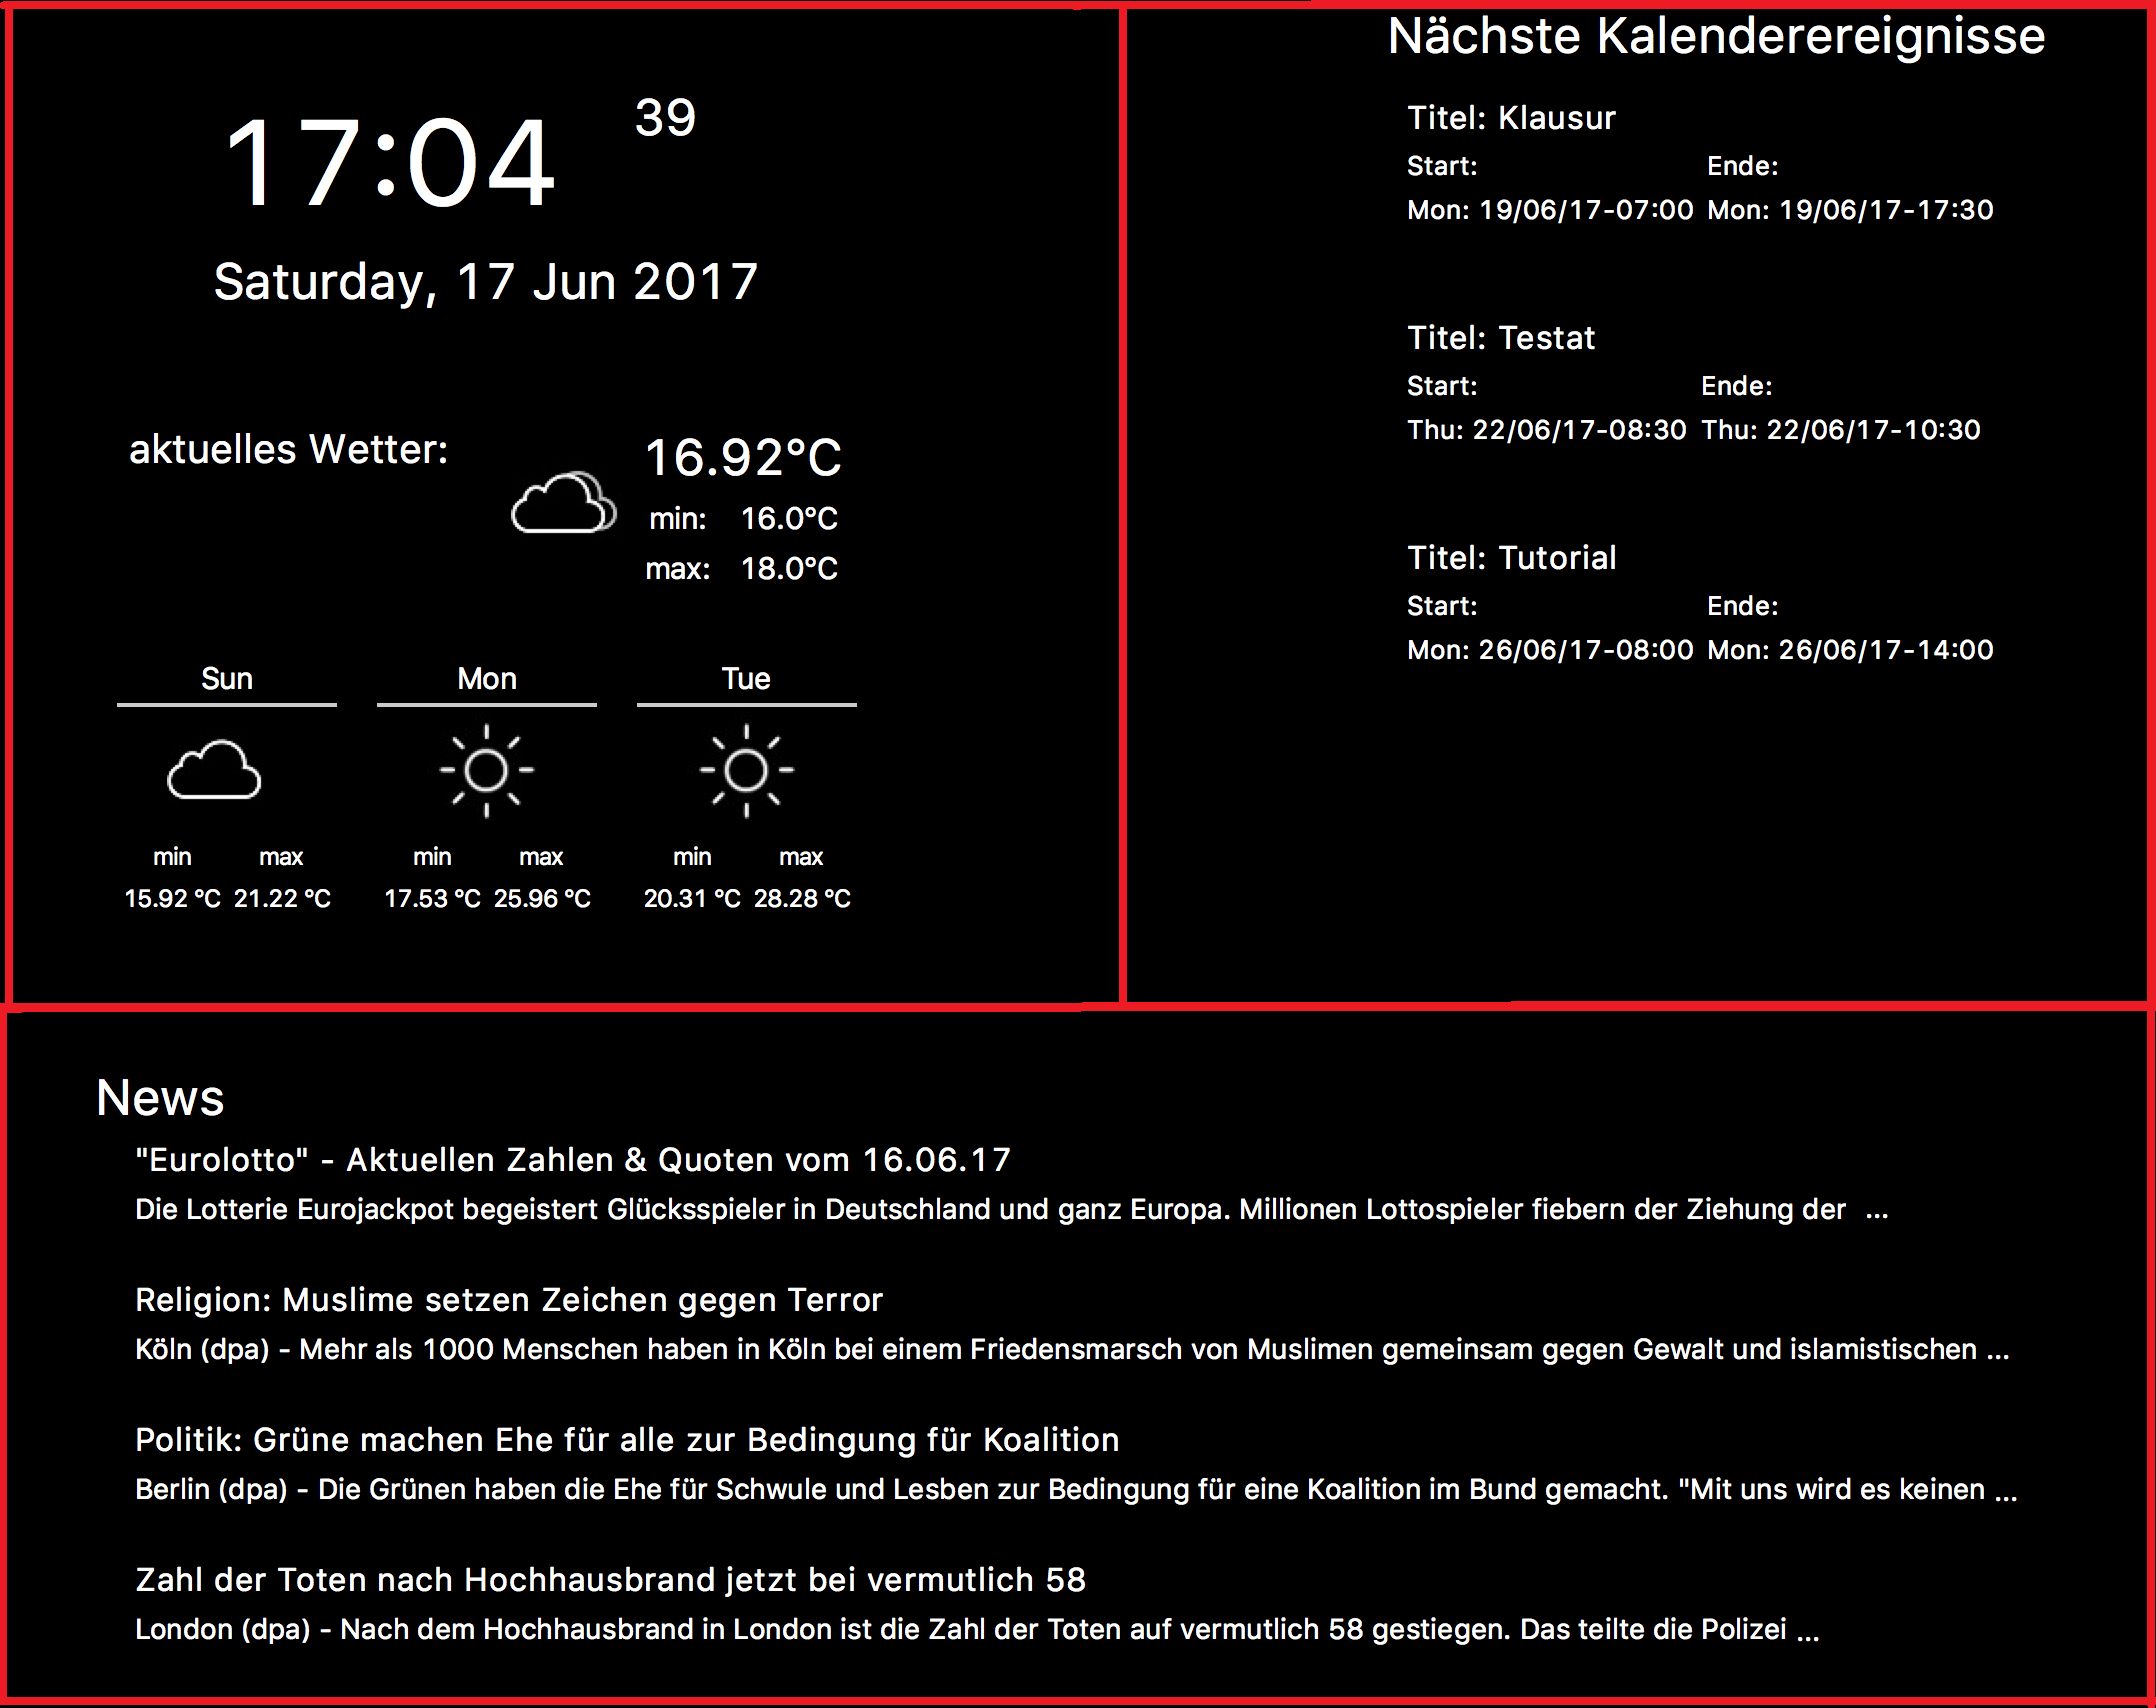
\includegraphics[width=0.7\linewidth]{bilder/grafOberflaeche}
	\caption[Benutzungsschnittstelle der SmartMirror-Anwendung]{Benutzungsschnittstelle der SmartMirror-Anwendung}
	\label{fig:grafoberflaeche}
\end{figure}


\subsection{Die SmartMirror-Anwendung}

Die Funktionalität der SmartMirror-Anwendung lässt sich am besten ausgehend von der Gestaltung der Benutzungsschnittstelle erfassen, die in \autoref{fig:grafoberflaeche} dargestellt wird. Die Darstellung lässt sich grob in drei Bereiche strukturieren: den oberen linken Bereich, den oberen rechten und den unteren Bereich. Oben links werden aktuelle Informationen konkret Uhrzeit, Datum und Wetterdaten angezeigt, während im rechten Bereich die nächsten Kalenderereignisse (bzw. ToDos) aufgeführt werden und im unteren Bereich aktuelle Neuigkeiten (News) angezeigt werden. 

\subsubsection*{Benutzungsschnittstelle}

Zur Gestaltung der Benutzungsschnittstelle wurde das Framework TkInter genutzt. Die Abkürzung steht für (\textbf{Tk Inter}face).  Durch Tkinter ist es mit Python möglich, Programme mit einer grafischen Benutzeroberfläche zu erstellen, die unter Windows, Mac OS und unter einigen Linux-Distributionen laufen. Bei TkInter handelt es sich, um das Standard GUI (Graphical User Interface) Package von Python. Es realisiert eine dünne objektorientierte Schicht über Tcl/Tk (Literatur). 

Zur Strukturierung der Oberfläche in die drei zuvor beschriebenen Bereiche wurde der Grid-Manager verwendet. Der Grid-Manager strukturiert Bedienelemente in einer Art Tabelle, die entsprechend in Reihen und Spalten angeordnet ist. Zur Anordnung werden 'row' und 'column' angegeben (vgl. \autoref{lst:structApplication}). Zeile 5 des Listings beschreibt, dass das \textit{GeneralInformation}-Frame, welches Uhrzeit, Datum und Wetterdaten anzeigt, in Zeile 0 und Spalte 0 angeordnet wird und in beide Dimensionen nur eine Zelle benötigt (\textit{rowspan=1, columnspan=1}). Der letzte Parameter in der Zeile (\textit{sticky=\grqq nse\grqq}) definiert die Ausrichtung der Subelement in dem Frame. Dabei steht jedes Zeichen (n, s, e) für eine Himmelsrichtung. Analog dazu wurden in den Zeilen 6 und 7 die weiteren Bereiche auf der Oberfläche angeordnet. In Zeile 7 legt \textit{\textit{columnspan=2}} fest, dass sich der Bereich über zwei Spalten erstreckt.

\begin{minipage}{\textwidth}
	\lstinputlisting[frame=single, language=python, style=myPython, escapeinside={(*}{*)}, caption={Hauptklasse der Anwendung}, label=lst:structApplication]{codesnippets/application.py}
\end{minipage}

Jeder Bereich ist als eigenes Frame realisiert. Während sowohl die Kalenderereignisse wie auch die News lediglich eine selbst implementierte Listendarstellung im Frame erfordern, ist das Frame, welches Uhrzeit, Datum und Wetterdaten anzeigt feingranularer strukturiert.

 
\subsubsection*{Struktur der Anwendung}

Bei der SmartMirror-Anwendung handelt es sich um eine Zwei-Schicht-Architektur (Literatur), die im Unterschied zu einer typischen Drei-Schicht-Architektur keine Geschäftslogik enthält (vgl. \autoref{fig:umldiagramClasses}). Die Darstellungsschicht (\textit{view}), die zuvor bereits von der Darstellungsseite  beschrieben wurde, greift auf eine weitere Schicht (\textit{model}) zu, die alle darzustellenden Daten enthält. Diese Daten werden zum Teil von externen Datenquellen importiert, wie in \autoref{fig:umldiagramClasses} dargestellt.

\begin{figure}
	\centering
	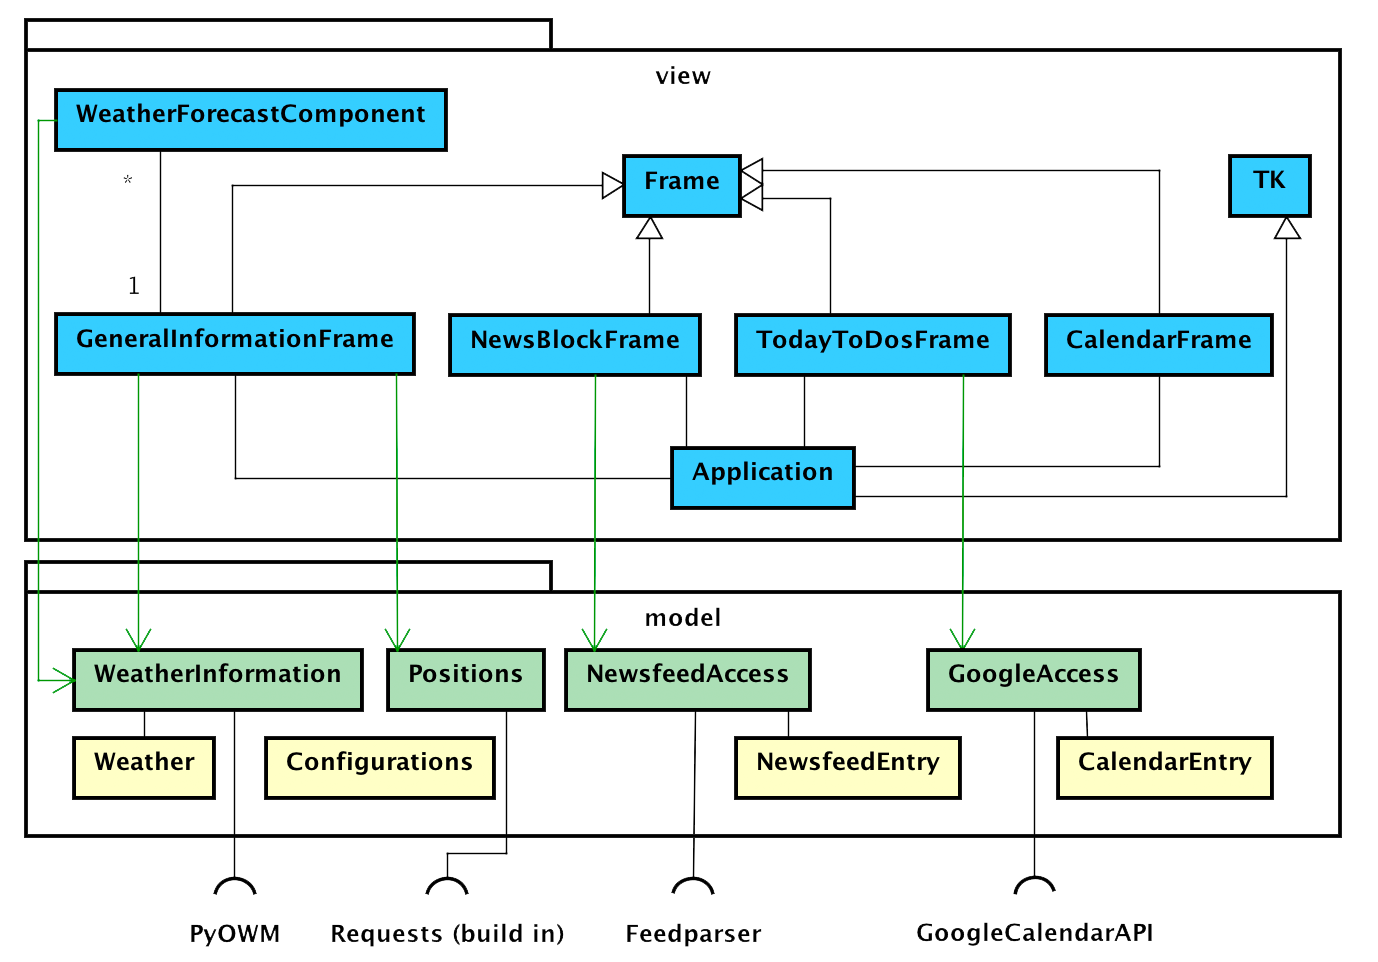
\includegraphics[width=0.7\linewidth]{bilder/umlDiagramNoBackground}
	\caption[UML-Diagramm: Klassenaufbau der Hauptapplikation]{UML-Diagramm: Klassenaufbau der Hauptapplikation}
	\label{fig:umldiagramClasses}
\end{figure}

\textcolor{green}{\textbf{Struktur passt nicht so ganz!!! - CalendarFrame rausschmeißen}}   

Die View-Schicht implementiert als wesentliches Element die Klasse \textit{Application}, die von \textit{Tk} erbt. 
\textit{Application} enthält, wie zuvor erwähnt die Frames \textit{NewsBlockFrame}, \textit{TodayToDosFrame}, sowie das \textit{GeneralInformationFrame}. Das \textit{GeneralInformationFrame} nutzt für die Darstellung die \textit{WeatherForeCastComponent}, während die aktuelle Urzeit und das Datum direkt über das Betriebssystem ermittelt und ausgegeben werden. Dies geschieht durch das Kommando \textit{time.strftime(\grq \%H:\%M\grq)} in Zeile 12 (vgl. \autoref{lst:structGeneralFrame}). Hierbei liefert die Methode die aktuelle Uhrzeit in dem Format Stunde:Minute zurück. In der darauf folgenden Zeile wird überprüft, ob sich die aktuell angezeigte Uhrzeit mit der neu Bestimmten übereinstimmt. Ist dies nicht der Fall, so wird in Zeile 14 über das Attribut \textit{$text=new\_ time$} die Aktualisierung vorgenommen.
Zeile 16 sorgt für den erneuten Methodenaufruf nach 200 Millisekunden.

\begin{minipage}{\textwidth}
	\lstinputlisting[frame=single, language=python, style=myPython, escapeinside={(*}{*)}, caption={GeneralInformation Frame},label=lst:structGeneralFrame]{codesnippets/frameExample.py}
\end{minipage}
 
 Die Model-Schicht importiert und hält die anzuzeigenden Daten vor, ebenso wie zentrale Informationen zur Darstellung, die als globale Variablen in \textit{Configurations} vorgehalten werden. \textit{Positions} ist eine Klasse, die über die IP-Adresse des WLAN-Interfaces die Position ermittelt, um daraus implizit den aktuellen Ort für die Wettervorhersage zu ermitteln. Diese Information benötigt die Klasse \textit{WeatherInformation}, um über die \textbf{Py}thon \textbf{O}pen \textbf{W}eather \textbf{M}ap (PyOWM) (vgl. Quelle) die aktuelle Wettervorhersage für den ermittelten Ort anzufragen. PyOWM selbst ist ein Python Wrapper zur Nutzung der Open Weather Map. Die erforderliche Kommunikation zur Ermittlung der Daten ist in (vgl. \autoref{fig:umldiagramClasses}) dargestellt.
 Die Klasse \textit{GeneralInformationFrame} fordert über die Methode \textit{getWeather} die Wetterdaten von der Klasse \textit{WeatherInformation} an. Diese startet über PyOWM eine Web-Anfrage bei der Open Weather Map. Nach Empfang der Daten legt \textit{WeatherInformation} die Informationen als \textit{Weather}-Daten im Model ab und stellt sie so dem \textit{GeneralInformationFrame} zu Verfügung. 


\begin{figure}
	\centering
	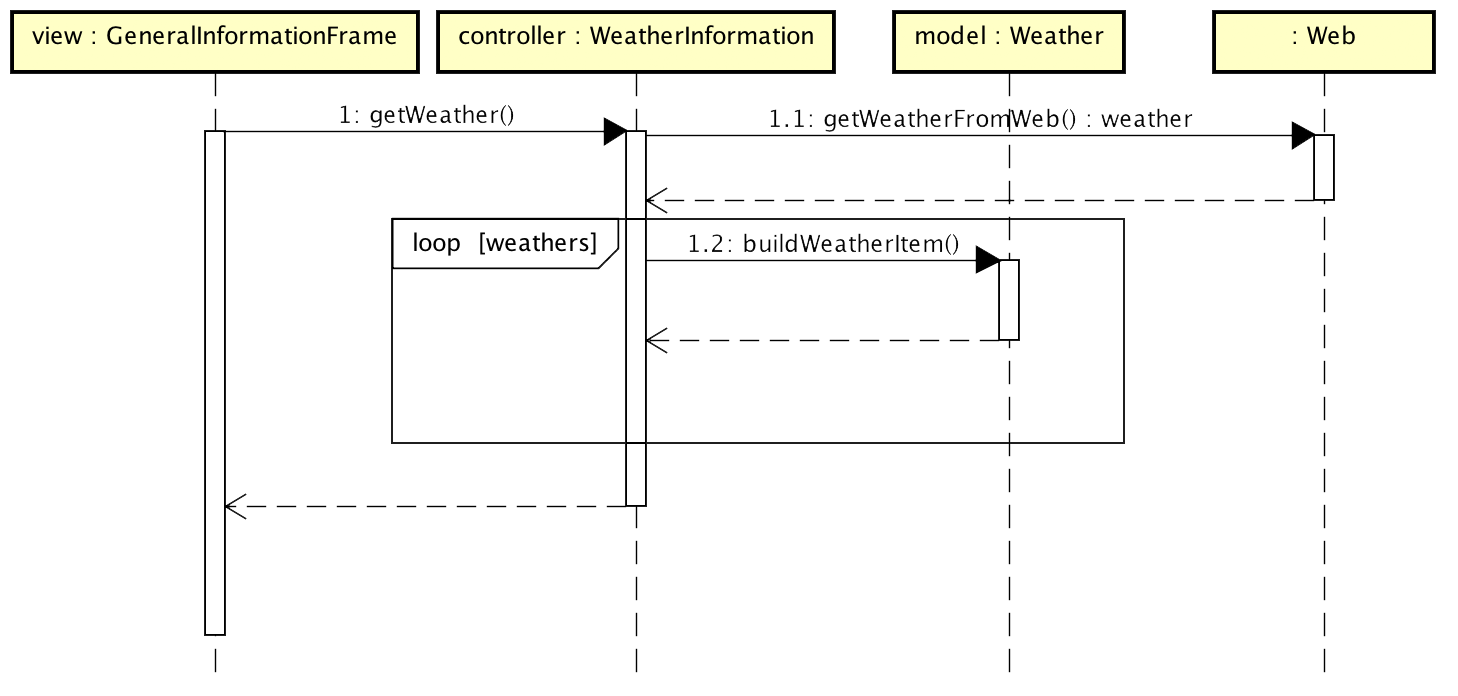
\includegraphics[width=0.7\linewidth]{bilder/sequenceDiagramGettingDataNoBackground}
	\caption{Sequenzdiagramm: Bezug von Daten aus dem Internet}
	\label{fig:sequenzDiagramData}
\end{figure}

\textcolor{green}{\textbf{Abbildung anpassen - MVC raus + Web durch Open Weather Map ersetzen}}   

Analog dazu stellt die Klasse \textit{NewsfeedAccess} Daten, die sie über den Feedparser \textcolor{green}{\textbf{konkretisieren!!!}} abfragt in Form von \textit{NewsFeedEntries} für den \textit{NewsBlockFrame} bereit. Ebenso ruft die Klasse \textit{GoogleAccess} die aktuellen Kalendereinträge über die GoogleCalendarAPI \textcolor{green}{\textbf{konkretisieren!!!}} 
ab und stellt sie als \textit{CalenderEntries} bereit.



\subsection{Das StartUp-Skript}

\section{Der SmartMirror im Einsatz}
\subsection{Inbetriebnahme}
\subsection{Showcase}

\section{Fazit und Ausblick}

\appendix
% anhang.tex
\chapter{Weitere Informationen}



%% ↑↑↑↑↑↑↑↑↑↑↑↑↑↑↑↑↑↑↑↑↑↑↑↑↑↑↑↑↑↑↑↑↑↑↑↑↑↑↑↑↑↑↑↑↑↑↑↑↑↑↑↑
%% ====================================================
%  Ab hier bis zum Ende nichts ändern!
%  Verzeichnisse werden automatisch anhand der in "einstellungen.tex" gewählten Optionen erstellt.
%% ========================
\ifthenelse{\boolean{PlatzsparendeVerzeichnisse}}{
\let\cleardoublepage\clearpage
}{}
\ifthenelse{\boolean{AbbildungsverzeichnisEinfuegen}}{
%Abbildungsverzeichnis
\listoffigures
\addcontentsline{toc}{chapter}{Abbildungsverzeichnis}
}{}
\ifthenelse{\boolean{TabellenverzeichnisEinfuegen}}{
%Tabellenverzeichnis
\listoftables
\addcontentsline{toc}{chapter}{Tabellenverzeichnis}
}{}
\ifthenelse{\boolean{AlgorithmenverzeichnisEinfuegen}}{
% Algorithmenverzeichnis
\listofalgorithms
\addcontentsline{toc}{chapter}{Algorithmenverzeichnis}
}{}
% Literaturverzeichnis
\bibliographystyle{alphadin}
\bibliography{literatur}
\addcontentsline{toc}{chapter}{\bibname}
% Erklaerung
%\cleardoublepage
%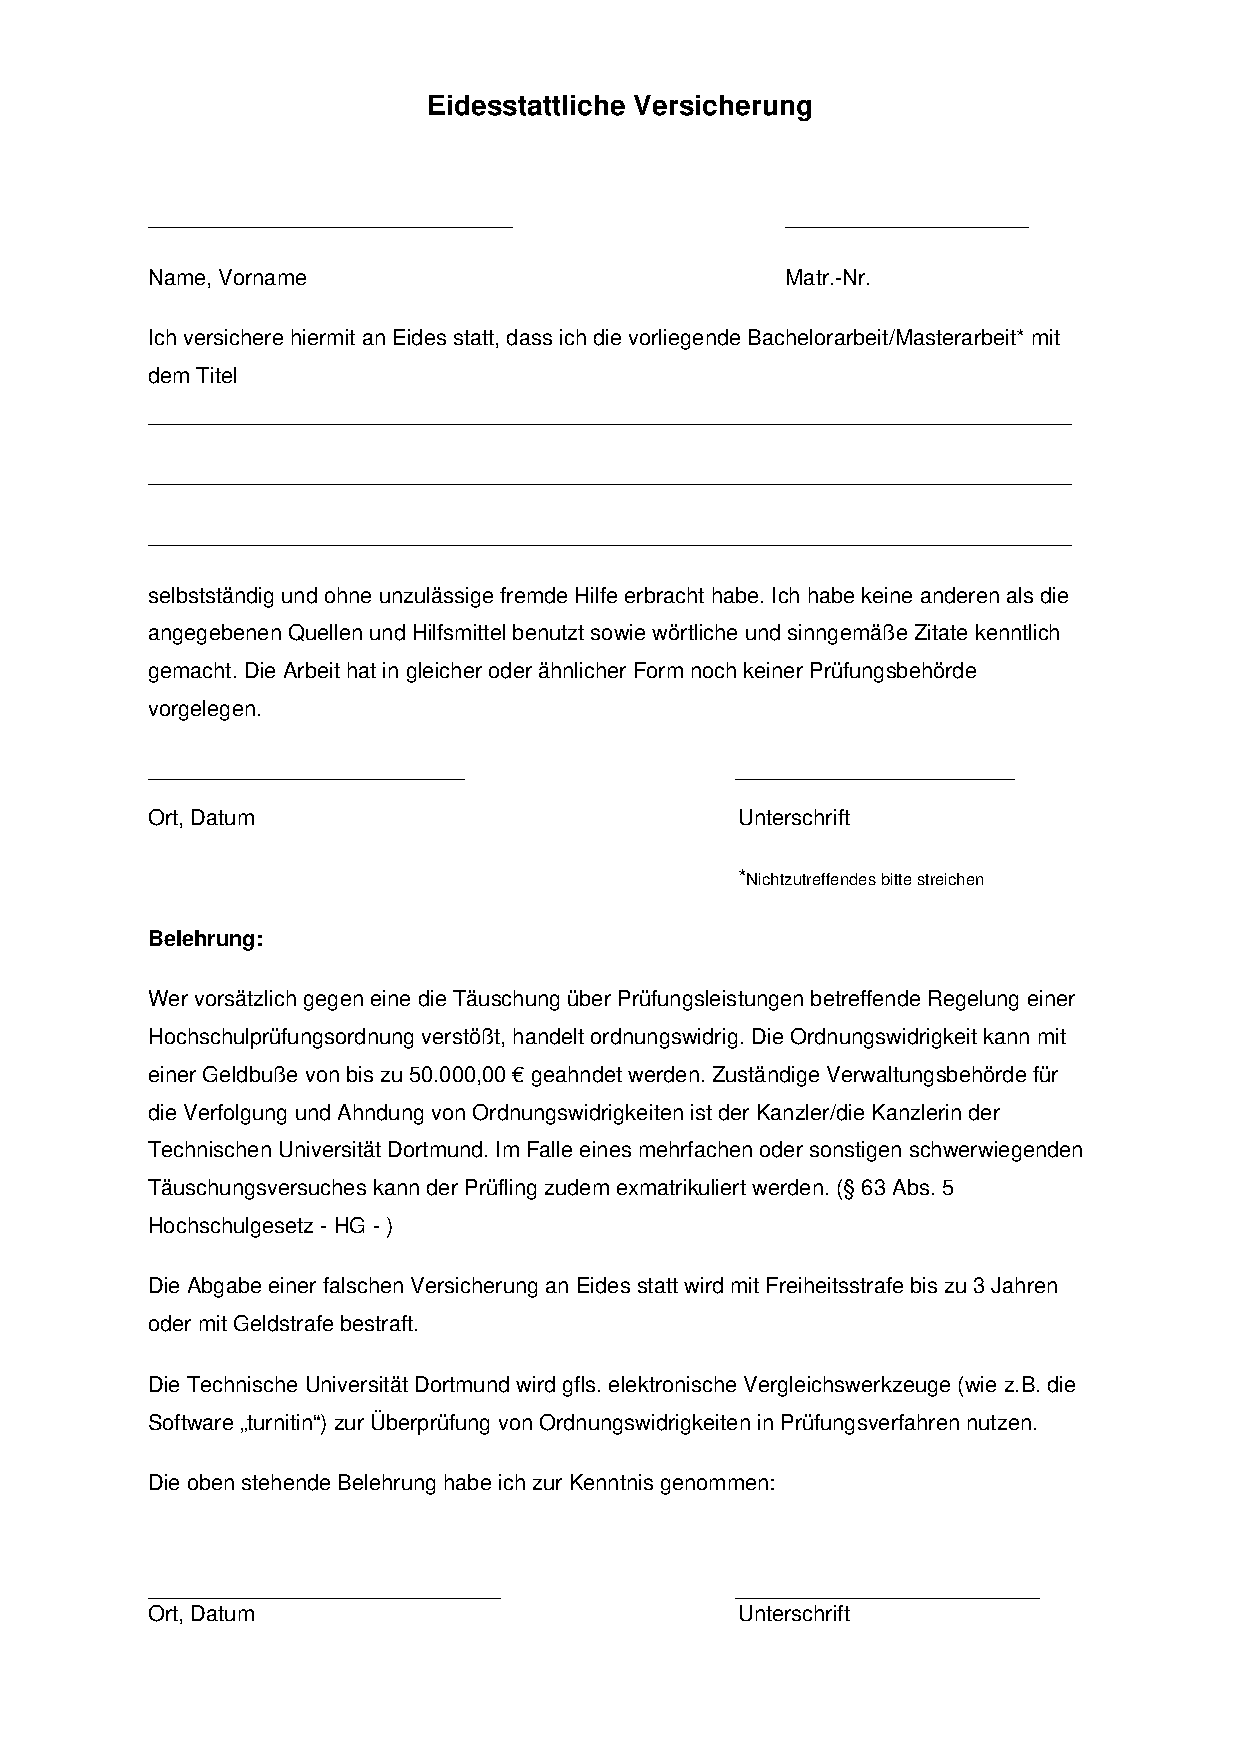
\includepdf[]{kapitel/Eidesstattliche_Versicherung.pdf}
\end{document}
